\newpage
\section{GÓC GIỮA ĐƯỜNG THẲNG VÀ MẶT PHẲNG. GÓC NHỊ DIỆN}
\subsection{Lý thuyết cần nhớ}
\subsubsection{Góc giữa đường thẳng và mặt phẳng}
Cho đường thẳng $d$ và mặt phẳng $(P)$, ta có định nghĩa sau
\begin{enumerate}
	\item Nếu đường thẳng $d$ vuông góc với mặt phẳng $(P)$ thì góc giữa $d$ và $(P)$ bằng $90^{\circ}$.
	\item Nếu đường thẳng $d$ không vuông góc với mặt phẳng $(P)$ thì góc giữa đường thẳng $d$ và mặt phẳng $(P)$ là góc giữa $d$ và hình chiếu $d$' của đường thẳng $d$ trên $(P)$.
\end{enumerate}
\begin{minipage}[c]{0.5\textwidth}
	\centering 
	$d$ vuông góc với $(P)$\\
	\begin{tikzpicture}[scale=0.8, font=\footnotesize,line join=round, line cap=round, >=stealth]
		\coordinate (A) at (2,2);
		\coordinate (B) at (7,2);
		\coordinate (D) at (0,0);
		\coordinate (C) at ($(B)+(D)-(A)$);
		\coordinate (E) at (3,0);
		\coordinate (F) at (3,-1);
		\coordinate (G) at (3,1);
		\coordinate (H) at (3,4);
		\draw[dashed] (E)--(G);
		\draw (E)--(F);
		\draw(A)--(B)--(C)--(D)--cycle;
		\draw(G)--(H) node [right] {$d$};
		\draw pic["$P$", draw,,angle radius=10mm]{angle=C--D--A};
	\end{tikzpicture}\\
	Góc giữa $d$ và $(P)$ bằng $90^\circ$.
\end{minipage}
\hfill 
\vline
\begin{minipage}[c]{0.5\textwidth}
	\centering 
	$d$ cắt $(P)$ nhưng không vuông góc với $(P)$\vskip .5cm
	\begin{tikzpicture}[scale=0.8, font=\footnotesize,line join=round, line cap=round, >=stealth]
		\coordinate (A) at (2,2);
		\coordinate (B) at (7,2);
		\coordinate (D) at (0,0);
		\coordinate (C) at ($(B)+(D)-(A)$);
		\coordinate (H) at (3,1);
		\coordinate (M) at (3,3);
		\coordinate (E) at (1,1);
		\coordinate (O) at (5,1);
		\coordinate (E') at (1.5,1);
		\coordinate (I) at (2,4);
		\coordinate (A') at (intersection of M--O and B--C);
		\path ($(O)!1.7!(A')$) coordinate (T);
		\draw(A)--(B)--(C)--(D)--cycle  (O)--(I) (A')--(T);
		\draw[dashed] (A')--(O);
		\draw(H)--(M) node [below left] {$d$};
		\draw(O)--(E') node [above right] {$d'$};
		\draw pic["$P$", draw,,angle radius=10mm]{angle=C--D--A};
		\foreach \x/\g in {M/60,H/-90,O/0}
		\fill[black] 	(\x) circle (1pt)
		($(\g:3mm)+(\x)$) node {$\x$};
		\draw pic["$\varphi$", draw,,angle radius=5mm]{angle=M--O--H};
	\end{tikzpicture}\\
	Góc giữa $d$ và $(P)$ bằng góc $MOH$.
\end{minipage}
\rule{\linewidth}{.5pt}
\begin{minipage}[c]{0.5\textwidth}
	\centering 
	$d$ song song với $(P)$\\
	\begin{tikzpicture}[scale=0.8, font=\footnotesize,line join=round, line cap=round, >=stealth]
		\coordinate (A) at (2,2);
		\coordinate (B) at (7,2);
		\coordinate (D) at (0,0);
		\coordinate (C) at ($(B)+(D)-(A)$);
		\coordinate (E) at (2,1);
		\coordinate (F) at (6,1);
		\coordinate (G) at (2,3);
		\coordinate (H) at (6,3);
		\coordinate (X) at (3,1);
		\coordinate (Y) at (3,3);
		\coordinate (Z) at (5,1);
		\coordinate (T) at (5,3);
		\draw[dashed] (X)--(Y) (Z)--(T);
		\draw(E)--(F) node [above] {$d'$};
		\draw(G)--(H) node [above] {$d$};
		\draw(A)--(B)--(C)--(D)--cycle;
		\draw pic["$P$", draw,,angle radius=10mm]{angle=C--D--A};
	\end{tikzpicture}\\
	Góc giữa $d$ và $(P)$ bằng $0^\circ$.
\end{minipage}
\hfill 
\vline
\begin{minipage}[c]{0.5\textwidth}
	\centering 
	$d$ nằm trong $(P)$\vskip .5cm
	\begin{tikzpicture}[scale=0.8, font=\footnotesize,line join=round, line cap=round, >=stealth]
		\coordinate (A) at (2,2);
		\coordinate (B) at (7,2);
		\coordinate (D) at (0,0);
		\coordinate (C) at ($(B)+(D)-(A)$);
		\coordinate (E) at (2,1);
		\coordinate (F) at (6,1);
		\coordinate (G) at (2,3);
		\coordinate (H) at (6,3);
		\coordinate (X) at (3,1);
		\coordinate (Y) at (3,3);
		\coordinate (Z) at (5,1);
		\coordinate (T) at (5,3);
		\draw(F)--(E) node [above right] {$d'$};
		\draw(F)--(E) node [below right] {$d \qquad (d'\equiv d)$};
		\draw(A)--(B)--(C)--(D)--cycle;
		\draw pic["$P$", draw,,angle radius=10mm]{angle=C--D--A};
	\end{tikzpicture}\\
	Góc giữa $d$ và $(P)$ bằng $0^\circ$.
\end{minipage}\\
\textbf{Nhận xét:} Góc giữa đường thẳng và mặt phẳng có số đo từ $0^\circ$ đến $90^\circ$.
\subsubsection{Góc nhị diện} 
\begin{itemize}
	\item \textbf{Nửa mặt phẳng:}\\
	Một đường thẳng nằm trong mặt phẳng chia mặt phẳng đó thành hai phần, mỗi phần được gọi là một nửa mặt phẳng và đường thẳng đó được gọi là bờ của mỗi nửa mặt phẳng này.
	\item \textbf{Góc nhị diện:}\\
	Góc nhị diện là hình gồm hai nửa mặt phẳng có chung bờ.\\
	\immini{
		Xét góc nhị diện gồm hai nửa mặt phẳng $(P)$ và $(Q)$ có chung bờ là đường thẳng $d$, kí hiệu là $[P,d,Q]$.\\
		Đường thẳng $d$ gọi là cạnh của góc nhị diện, mỗi nửa mặt phẳng $(P)$ và $(Q)$ gọi là một mặt của góc nhị diện.\\
		\textbf{Chú ý:} Góc nhị diện còn được kí hiệu là $[M,d,N]$ với $M$, $N$ lần lượt là các điểm thuộc các nửa mặt phẳng $(P)$, $(Q)$ nhưng không thuộc đường thẳng $d$.}{	 
		\begin{tikzpicture}
			\def\a{3}
			\path 	(0:0) coordinate (A)
			++(10:\a) coordinate (D)
			++(90:\a) coordinate (C)
			($(A)+(C)-(D)$) coordinate (B)
			++(-10:2*\a/3) coordinate (E)
			++(-90:\a) coordinate (F)	
			($(A)!0.5!(B)$) coordinate (I)%k là tỉ số AB' trên AB
			(intersection of A--D and E--F) coordinate (O);%giao điểm O
			\draw[thick] (B)--(E)--(F)--(A)	(O)--(D)		(B)-- (C)--(D);
			\draw[thick] (A)--(B) node at (I) [left] {$d$};
			\draw[dashed] (A)--(O);
			\draw pic["$Q$", draw,,angle radius=10mm]{angle=B--C--D};
			\draw pic["$P$", draw,,angle radius=10mm]{angle=B--E--F};
	\end{tikzpicture}}
\end{itemize}
\subsubsection{Góc phẳng nhị diện}
Trong không gian, cho góc nhị diện. Một góc có đỉnh thuộc cạnh của góc nhị diện, hai cạnh của góc đó lần lượt thuộc hai mặt nhị diện và cùng vuông góc với cạnh của góc nhị diện, được gọi là góc phẳng nhị diện của góc nhị diện đã cho.\\
\immini{
	Cho góc nhị diện $[P, d, Q]$.\\
	Lấy $O$ thuộc $d$, hai tia $Ox$, $Oy$ lần lượt nằm trên hai nửa mặt phẳng $(P)$, $(Q)$ và cùng vuông góc với $d$.\\
	Khi đó góc $xOy$ là góc phẳng nhị diện của góc nhị diện $[P, d, Q]$.\\
	\textbf{Nhận xét:} Cạnh của góc nhị diện luôn vuông góc với mặt phẳng chứa góc phẳng nhị diện của góc nhị diện đó.}{
	\begin{tikzpicture}
		\def\a{3}
		\path 	(0:0) coordinate (A)
		++(0:\a) coordinate (B)
		++(30:\a) coordinate (C)
		($(A)+(C)-(B)$) coordinate (D)
		++(70:\a) coordinate (F)
		($(A)+(F)-(D)$) coordinate (E)
		($(A)!0.5!(D)$) coordinate (O)
		++(0:5*\a/6) coordinate (Y)
		($(O)+(70:2*\a/3)$) coordinate (X) 
		;
		\draw[thick] (A)--(B)--(C)--(D)--(F)--(E)--(A)--(D);
		\draw (O)--(X) node [below left] {$x$};
		\draw (O)--(Y) node [below left] {$y$};
		\draw pic[ draw,,angle radius=5mm]{angle=Y--O--X};
		\draw pic["$P$", draw,,angle radius=10mm]{angle=E--F--D};
		\draw pic["$Q$", draw,,angle radius=10mm]{angle=D--C--B};
		\draw pic[draw,angle radius=3mm]{right angle=X--O--A};
		\draw pic[draw,angle radius=3mm]{right angle=Y--O--A};
		\foreach \x/\g in {O/-70}
		\fill[black] 	(\x) circle (1pt)
		($(\g:3mm)+(\x)$) node {$\x$};
\end{tikzpicture}}
\subsubsection{Số đo của góc nhị diện} 
\begin{enumerate}
	\item Số đo của một góc phẳng nhị diện được gọi là số đo của góc nhị diện đó.
	\item Nếu số đo góc phẳng nhị diện bằng $90^{\circ}$ thì góc nhị diện đó gọi là góc nhị diện vuông.
\end{enumerate}
\textbf{Nhận xét:} Số đo của góc nhị diện từ $0^{\circ}$ đến $180^{\circ}$.
\subsection{Phân loại và phương pháp giải toán}
\begin{dang}{Góc giữa đường thẳng và mặt phẳng}
	Đưa bài toán về xác định góc giữa hai đuờng thẳng, cụ thể là góc giữa đường thẳng và hình chiếu của nó trên mặt phẳng.
\end{dang}
%%%=============VD_1=============%%%
\begin{vd}%[1H8H6-1]%[Dự án D - đợt 2 NH24-25- Thy Nguyen Vo Diem]
	Cho hình chóp $S.ABCD$ có $SA \perp(ABCD)$, $AB \perp AD$, $SA=AD=a \sqrt{3}$, $AB=a$. Tính số đo của
	\begin{enumerate}
		\item Góc giữa đường thẳng $SB$ và mặt phẳng $(ABCD)$.
		\item Góc giữa đường thẳng $SD$ và mặt phẳng $(SAB)$.
	\end{enumerate}
	\loigiai
	{
		\immini{\begin{enumerate}
				\item 	Vì $SA \perp(ABCD)$ nên $AB$ là hình chiếu của $SB$ trên $(ABCD)$.\\
				Suy ra góc giữa đường thẳng $SB$ và mặt phẳng $(ABCD)$ bằng góc giữa $SB$ và $AB$, hay bằng $\widehat{SBA}$.\\
				Trong tam giác vuông $S A B$ có
				$$
				\tan \widehat{SBA}=\dfrac{SA}{A B}=\frac{a \sqrt{3}}{a}=\sqrt{3}$$ nên $\widehat{S B A}=60^{\circ}$.\\
				Suy ra góc giữa đường thẳng $SB$ và mặt phẳng $(ABCD)$ bằng $60^{\circ}$.
				\item Vì $SA \perp(ABCD)$ và $AD \subset(ABCD)$ nên $SA \perp AD$.\\
				Mà $AD \perp AB$ và $SA$, $AB$ cắt nhau trong mặt phẳng $(SAB)$ nên $AD \perp(SAB)$.\\ Suy ra $SA$ là hình chiếu của $SD$ trên $(SAB)$.\\
				Khi đó góc giữa đường thẳng $SD$ và mặt phẳng $(SAB)$ bằng góc giữa $SD$ và $SA$, hay bằng $\widehat{DSA}$.\\
				Vì tam giác $DSA$ vuông cân tại $A$ nên $\widehat{DSA}=45^{\circ}$.\\
				Vậy góc giữa đường thẳng $SD$ và mặt phẳng $\left(SAB\right)$ bằng $45^{\circ}$.
		\end{enumerate}}{
			\begin{tikzpicture}[scale=0.7, font=\footnotesize, line join=round, line cap=round, >=stealth]
				\def\a{4}
				\def\h{4}
				\path 	(0:0) coordinate (A)
				++(0:\a) coordinate (D)
				++(-130:\a/2) coordinate (C)
				($(A)+(C)-(D)$) coordinate (B)
				($(A)+(90:\h)$) coordinate (S)
				(intersection of A--C and B--D) coordinate (O);%giao điểm O
				\draw[dashed] 	(B)--(A)--(D)	(A)--(S);
				\draw 			(B)-- (C)--(D)
				(B)--(S)	(C)--(S)	(D)--(S);
				\foreach \x/\g in {A/135,B/-135,C/-45,D/45,S/90}
				\fill[black] 	(\x) circle (1.5pt)
				($(\g:3mm)+(\x)$) node {$\x$};
				\draw pic[draw,angle radius=3mm]{right angle=D--A--S};%Theo chiều dương
			\end{tikzpicture}
		}
	}
\end{vd}
%%%=============================%%%

%%%=============VD_2=============%%%
\begin{vd}%[1H8H6-1]%[Dự án D - đợt 2 NH24-25- Thy Nguyen Vo Diem]
	Cho hình chóp $S.ABCD$ có đáy $ABCD$ là hình vuông (hoặc hình chữ nhật). Gọi $I$ là trung điểm của $AB$, biết $SI\perp (ABCD)$. Tìm hình chiếu của chân đường vuông góc $I$ lên mặt phẳng $(SCD)$ và xác định góc giữa $SI$ và mặt phẳng $(SCD)$.
	\loigiai{
		\immini
		{
			Gọi $K$ là trung điểm của $CD\Rightarrow IK\perp CD$. \\[4pt]
			Kẻ $IH\perp SK$ tại $H$.\tagEX{1}
			Ta có $\heva{& CD\perp IK \\ & CD\perp SI}\Rightarrow CD\perp (SIK)\Rightarrow CD\perp IH$. \tagEX{2}
			Từ $(1)$, $(2)\Rightarrow IH\perp (SCD)$.\\
			Hay $SH$ là hình chiếu của $SI$ trên mặt phẳng $(SCD)$.\\
			Vậy góc giữa $SI$ và mặt phẳng $(SCD)$ bằng $\widehat{ISH}=\widehat{ISK}$.
		}
		{
			\begin{tikzpicture}[scale=0.65, font=\footnotesize, line join=round, line cap=round, >=stealth]
				\path (0,0) coordinate (A)
				(-2,-2) coordinate (B)
				(5,0) coordinate (D);
				\coordinate (C) at ($(B)+(D)-(A)$);
				\coordinate (I) at ($(A)!1/2!(B)$);
				\coordinate (S) at ($(I)+(0,5)$);
				\coordinate (K) at ($(C)!1/2!(D)$);
				\coordinate (H) at ($(S)!0.65!(K)$);
				\draw (S)--(B)--(C)--(D)--(S)--(C) (S)--(K);
				\draw[dashed] (S)--(A)--(B) (A)--(D) (S)--(I)--(K) (I)--(H);
				\foreach \i/\g in {S/90, A/170, B/-90, C/-90, D/0,I/-90,H/0,K/0}
				\fill (\i) circle (1pt)+(\g:3mm) node {$\i$};
				\path
				pic[draw,angle radius=5]{right angle=I--H--K}
				pic[draw,angle radius=5]{right angle=I--K--C}
				pic[draw,angle radius=5]{right angle=S--I--B}
				;
			\end{tikzpicture}
		}
	}
\end{vd}
%%%=============================%%%

%%%=============VD_3=============%%%
\begin{vd}%[1H8H6-1]%[Dự án D - đợt 2 NH24-25- Thy Nguyen Vo Diem]
	Cho hình chóp $S.ABCD$ có đáy là hình thang vuông tại $A$ và $B$, $AB=BC=a$, $AD=2a$. Cạnh bên $SA=a\sqrt{2}$ và vuông góc với đáy. Tính góc giữa đường thẳng $SB$ và mặt phẳng $(SAC)$.
	\loigiai{
		\immini{Gọi $I$ là trung điểm $AD$.\\
			Lúc đó $ABCI$ là hình vuông, suy ra $BI\perp AC$ (tại $O$).\\
			Mà $SA\perp (ABCD)$ nên $BI\perp SA$.\\
			Do đó $BI\perp (SAC)$ tại $O$ nên $SO$ là hình chiếu vuông góc của $SB$ lên $(SAC)$, suy ra $(SB,(SAC))=(SB,SO)=\widehat{BSO}$.\\
			Trong $\triangle SBO$ có $\sin\widehat{BSO}=\dfrac{BO}{SB}=\dfrac{\dfrac{BI}{2}}{\sqrt{SA^2+AB^2}}=\dfrac{\sqrt{6}}{6}$.\\
			Suy ra $(SB,(SAC))=\arcsin\dfrac{\sqrt{6}}{6}\approx 24^{\circ}$.
		}{\begin{tikzpicture}[>=stealth, line join=round, line cap=round,scale=0.7,font=\footnotesize]
				\path
				(0,0) coordinate (A)--++(-2,-2) coordinate (B)--++(4,0) coordinate (C)--++(5,2) coordinate (D)
				(A)--++(0,3) coordinate (S);
				\coordinate (I) at ($(A)!0.5!(D)$);
				\coordinate (O) at (intersection of A--C and B--I);
				\draw (S)--(B)--(C)--(D)--(S)--(C);
				\draw[dashed] (S)--(A)--(B) (C)--(A)--(D) (C)--(I)--(B) (S)--(O);
				\foreach \i/\g in {S/90, A/170, B/-90, C/-90, D/0, O/-90,I/90}
				\fill (\i) circle (1pt)+(\g:3mm) node {$\i$};
				\path
				pic[draw,angle radius=5]{right angle=A--B--C}
				pic[draw,angle radius=5]{right angle=B--A--D}
				pic[draw,angle radius=5]{right angle=S--A--D}
				;
			\end{tikzpicture}
		}
	}
\end{vd}
%%%=============================%%%

\begin{dang}{Góc nhị diện}
	Xác định vị trí của góc phẳng nhị diện (nằm trên mặt phẳng vuông góc với cạnh của góc nhị diện) rồi tính số đo của góc phẳng nhị diện đó.
\end{dang}

%%%=============VD_1=============%%%
\begin{vd}%[1H8H6-2]%[Dự án D - đợt 2 NH24-25- Thy Nguyen Vo Diem]
	Cho hình chóp $S.ABCD$ có $SA\perp(ABCD)$, đáy $ABCD$ là hình thoi cạnh $a$ và $AC=a$. Tính số đo của mỗi góc nhị diện sau:
	\begin{listEX}[2]
		\item $[B,SA,C]$;
		\item $[S,DA,B]$.
	\end{listEX}
	\loigiai{
		\immini{ \begin{enumerate}
				\item Vì $SA\perp(ABCD)$ nên $SA\perp AB$, $SA\perp AC$.\\
				Suy ra góc $BAC$ là góc phẳng nhị diện của góc nhị diện $[B, SA, C]$.\\
				Do $AC=AB=BC=a$ nên tam giác $ABC$ đều, suy ra $\widehat{BAC}=60^{\circ}$.\\
				Vậy góc nhị diện $[B,SA,C]$ có số đo bằng $60^{\circ}$.
				\item Ta có $SA \perp DA$ và $BA \perp DA$ nên góc $SAB$ là góc phẳng nhị diện của góc nhị diện $[S,DA,B]$.\\
				Vậy góc nhị diện $[S, DA, B]$ có số đo bằng $90^{\circ}$ do $\widehat{SAB}=90^{\circ}$.
		\end{enumerate}}{
			\begin{tikzpicture}[scale=0.7, font=\footnotesize, line join=round, line cap=round, >=stealth]
				\def\a{4}
				\path 	(0:0) coordinate (A)
				++(0:\a) coordinate (D)
				++(-130:\a/2) coordinate (C)
				($(A)+(C)-(D)$) coordinate (B)
				($(A)+(90:\a)$) coordinate (S)
				(intersection of A--C and B--D) coordinate (O);%giao điểm O
				\draw[dashed] (C)--(A)	(B)--(A)--(D)	(A)--(S);
				\draw			(B)-- (C)--(D)
				(B)--(S)	(C)--(S)	(D)--(S);
				\foreach \x/\g in {A/135,B/-135,C/-45,D/45,S/90}
				\fill[black] 	(\x) circle (1pt)
				($(\g:3mm)+(\x)$) node {$\x$};
	\end{tikzpicture}}}
\end{vd}
%%%=============================%%%

%%%=============VD_2=============%%%
\begin{vd}%[1H8H6-2]%[Dự án D - đợt 2 NH24-25- Thy Nguyen Vo Diem]
	Cho hình lập phương $ABCD.A'B'C'D'$ có cạnh bằng $a$.
	\begin{enumerate}
		\item Tính góc tạo bởi hai mặt phẳng $\left(ACD'\right)$ và $(ABCD)$.
		\item Tính số đo của góc nhị diện $\left[D',AC,B\right]$.
	\end{enumerate}
	\loigiai
	{
		\immini
		{
			\begin{enumerate}
				\item Gọi $I$ là giao điểm của $AC$ và $BD$. Ta có $DI\perp AC$, $DD'\perp AC$ nên $AC\perp\left(DD'I\right)$. Suy ra $AC\perp D'I$.\\
				Vì $\left\{\begin{aligned}&\left(ACD'\right)\cap(ABCD)=AC\\&D'I\subset\left(ACD'\right), D'I\perp AC\\&DI\subset(ABCD), DI\perp AC
				\end{aligned}\right.$ nên góc tạo bởi hai mặt phẳng $\left(ACD'\right)$ và $(ABCD)$ bằng góc tạo bởi hai đường thẳng $D'I$ và $DI$, chính là $\widehat{D'ID}$ (do $D'D\perp DI$).\\
				Ta có $DI=\dfrac{BD}{2}=\dfrac{a\sqrt{2}}{2}$.
			\end{enumerate}
		}
		{
			\begin{tikzpicture}[line cap=round, line join=round, font=\footnotesize, >=stealth, scale=1]
				\def\a{3}
				\path (0,0) coordinate (A) (-140:{.5*\a}) coordinate (B) (\a,0) coordinate (D) ($(D)-(A)+(B)$) coordinate (C) ($(A)!0.5!(C)$) coordinate (I);
				\foreach\x in {A,B,C,D} \path ($(\x)+(0,\a)$) coordinate (\x');
				\draw (C') --(B') --(A') --(D') --(C') --(C) --(D') --(D) --(C) --(B) --(B');
				\draw[dashed] (A')--(A)--(B) (C)--(A)--(D')--(I)--(D)--(A) (I)--(B);
				\foreach\x/\y in {A/180,B/-135,C/-45,D/0,A'/135,B'/180,C'/100,D'/45,I/-100}\fill (\x) circle (1pt)+(\y:0.3) node{$\x$};
			\end{tikzpicture}
		}
		\vspace*{-.5cm}
		\begin{enumerate}
			\item[] Trong tam giác $D'ID$ vuông tại $D$ ta có $\tan\widehat{D'ID}=\dfrac{DD'}{DI}=\dfrac{a}{\dfrac{a\sqrt{2}}{2}}=\sqrt{2}$.\\
			Suy ra $\widehat{D'ID}\approx 54{,}7^\circ$.\\
			Vậy góc tạo bởi hai mặt phẳng $\left(ACD'\right)$ và $(ABCD)$ gần bằng $54{,}7^{\circ}$.
			\setcounter{enumi}{1}
			\item Do $ID'\perp AC$, $IB\perp AC$ nên $\widehat{BID'}$ là góc phẳng nhị diện $\left[D',AC,B\right]$.\\
			Ta có $\widehat{BID'}=180^\circ-\widehat{D'ID}\approx 180^\circ-54{,}7^\circ=125{,}3^\circ$.\\
			Vậy số đo của góc nhị diện $\left[D',AC,B\right]$ gần bằng $125{,}3^\circ$.
		\end{enumerate}
	}
\end{vd}
%%%=============================%%%

%%%=============VD_3=============%%%
\begin{vd}%[1H8H6-2]%[Dự án D - đợt 2 NH24-25- Thy Nguyen Vo Diem]
	Cho tứ diện $S.ABC$ có các cạnh $SA$, $SB$, $SC$ đôi một vuông góc và $SA=SB=SC=1$. Gọi $\varphi$ là số đo của góc nhị diện $[S,BC,A]$. Tính $\cos\varphi$.
	\loigiai
	{
		\immini
		{
			Ta có $SA\perp SB$, $SA\perp SC$ nên $SA\perp(SBC)$.\\
			Tam giác $SBC$ có $SB=SC=1$ nên $SBC$ là tam giác cân tại $S$.\\
			Gọi $M$ là trung điểm của $BC$, khi đó $SM\perp BC$. Thêm nữa, $BC\perp SA$ (do $SA\perp(SBC)$). Cho nên $BC\perp(SAM)$, suy ra $BC\perp AM$.\\
			Do $\left\{\begin{aligned}&(SBC)\cap(ABC)=BC\\&SM\subset(SBC), SM\perp BC\\&AM\subset(ABC), AM\perp BC
			\end{aligned}\right.$ nên góc nhị diện $[S,BC,A]$ bằng góc $\widehat{SMA}=\varphi$ (do $SA\perp SM$).\\
			Tam giác $SBC$ vuông cân tại $S$ nên $BC=SB\sqrt{2}=\sqrt{2}$.\\
			Suy ra $SM=\dfrac{BC}{2}=\dfrac{\sqrt{2}}{2}$.
		}
		{
			\begin{tikzpicture}[line cap=round,line join=round,font=\footnotesize,scale=1]
				\path (0:0) coordinate(S) (0:3) coordinate(B) (-60:2) coordinate(C) (90:3) coordinate(A) ($(C)!.5!(B)$) coordinate(M);
				\draw (A)--(S)--(C)--(B)--cycle (A)--(C) (A)--(M);
				\draw[dashed] (B)--(S)--(M);
				\foreach \d/\g in {A/90, B/0, C/-90, S/180, M/-40}
				\fill (\d) circle(1pt) node[shift={(\g:.3)}]{$\d$};
				\path pic[draw,angle radius=.15cm]{right angle=A--S--B} pic[draw,angle radius=.15cm]{right angle=A--S--C} pic[draw,angle radius=.15cm]{right angle=S--M--C} pic[draw,angle radius=.15cm]{right angle=A--M--B};
			\end{tikzpicture}
		}
		\noindent
		Trong tam giác $SAM$ vuông tại $S$ ta có $AM=\sqrt{SA^2+SM^2}=\sqrt{1^2+\left(\dfrac{\sqrt{2}}{2}\right)^2}=\dfrac{\sqrt{6}}{2}$.\\
		Khi đó, $\cos\varphi=\cos\widehat{SMA}=\dfrac{SM}{AM}=\dfrac{\sqrt{2}}{2}\cdot\dfrac{2}{\sqrt{6}}=\dfrac{1}{\sqrt{3}}$.
	}
\end{vd}
%%%=============================%%%
\begin{dang}{Ứng dụng thực tế}
	
\end{dang}

%%%=============VD_1=============%%%
\begin{vd}%[1H8V6-7]%[Dự án D - đợt 2 NH24-25- Thy Nguyen Vo Diem]
	Cánh cửa có dạng hình chữ nhật $BCMN$ và khung cửa có dạng hình chữ nhật $ABCD$, ở đó $AB=BN$. Góc mở cửa là góc nhị diện $[A, BC, N]$. Biết chiều rộng $BN$ của cửa là $1,2\mathrm{~m}$. Khi góc mở cửa có số đo bằng $60^{\circ}$ thì khoảng cách giữa $A$ và $N$ bằng bao nhiêu?
	\loigiai{
		\immini{Vì $AB\perp BC$ và $NB\perp BC$ nên góc $ABN$ là góc phẳng nhị diện của góc nhị diện $[A, BC, N]$.\\
			Vì góc mở cửa bằng $60^{\circ}$ nên số đo góc nhị diện $[A, BC, N]$ bằng $60^{\circ}$, suy ra $\widehat{ABN}=60^{\circ}$.\\
			Xét tam giác $ABN$ cân tại $B$ có $BA=BN=1,2\mathrm{~m}$ và $\widehat{ABN}=60^{\circ}$.\\
			Khi đó tam giác $ABN$ đều, suy ra $AN=1,2\mathrm{~m}$, hay khoảng cách giữa $A$ và $N$ bằng $1,2\mathrm{~m}$.}{
			\begin{tikzpicture}
				\def\a{3}
				\path 	(0:0) coordinate (A)
				++(0:\a) coordinate (B)
				++(90:\a) coordinate (C)
				($(A)+(C)-(B)$) coordinate (D)
				($(A)+(-20:\a/3)$) coordinate (N)
				++(90:\a) coordinate (M)
				(intersection of A--B and M--N) coordinate (O);
				\draw[thick] (A)--(D)--(C)--(B)--(N)--(M)--(C) (A)--(O);
				\foreach \x/\g in {A/135,B/0,C/0,D/45,M/180,N/-90}
				\fill 	(\x) circle (0.11pt)
				($(\g:3mm)+(\x)$) node {$\x$};
				\fill[gray] (M) -- (N) -- (B) -- (C) -- cycle;
	\end{tikzpicture}}}
\end{vd}
%%%=============================%%%

%%%=============VD_2=============%%%
\begin{vd}%[1H8V6-7]%[Dự án D - đợt 2 NH24-25- Thy Nguyen Vo Diem]
	Một máy nước nóng sử dụng năng lượng mặt trời như ở Hình 20 có các ống hấp nhiệt chân không dài $1{,}8$ m được đặt trên sân thượng của một toà nhà. Khi tia nắng mặt trời chiếu vuông góc với sân thượng, bóng nắng của các ống hấp nhiệt chân không trên mặt sân dài $1{,}2$ m. Các ống hấp nhiệt chân không đó tạo với mặt sân thượng một góc bằng bao nhiêu độ (làm tròn kết quả đến hàng đơn vị)?
	\begin{center}
		\includegraphics[scale=0.15]{Images/maynuocnong}
	\end{center}
	\loigiai{
		\immini{\hfil Vẽ $OA$ biểu diễn cho ống hấp nhiệt chân không, $OH$ biểu diễn bóng nắng (hình chiếu vuông góc do tia nắng chiếu vuông gớc với mặt sân) của ống đó trên mặt sân. Như vậy góc giữa ống hấp nhiệt chân không với mặt sân bằng $\widehat{AOH}$. Ta có \\
			$\cos\widehat{AOH}=\dfrac{OH}{OA}=\dfrac{1{,}2}{1{,}8}=\dfrac{2}{3}\Rightarrow\widehat{AOH}\approx 48^{\circ}$.\\
		}
		{\begin{tikzpicture}[scale=0.8, font=\footnotesize, line join=round, line cap=round, >=stealth]
				
				\path
				(0,0) coordinate (O)%khai báo điểm
				($(O)+(0:5)$) coordinate (H)
				($(H)+(90:3)$) coordinate (A)
				;
				\draw
				(A)--(O)--(H)--(A)
				;
				\draw (O)--(H) node[below,sloped,pos=0.5] {1{,}2 m};
				\draw (O)--(A) node[above,sloped,pos=0.5] {1{,}8 m};
				\foreach \x/\g in {A/90,O/180,H/-90}
				\fill (\x) circle (1pt)+(\g:.4)node{$\x$};
		\end{tikzpicture}}
		Vậy góc giữa ống hấp nhiệt chân không với mặt sân thượng bằng khoảng $48^{\circ}$.
	}
\end{vd}
%%%=============================%%%
\subsection{Bài tập rèn luyện}
\ind{PHẦN I.} \inden{Câu trắc nghiệm nhiều phương án lựa chọn. Mỗi câu hỏi học sinh chỉ chọn một phương án.}\\
\setcounter{ex}{0}
\Opensolutionfile{ans}[ans/1H8-Bai5-TN]
%%%=============EX_1=============%%%
\begin{ex}%[1H8N6-1]%[Dự án D - đợt 2 NH24-25- Thy Nguyen Vo Diem]
	Cho hai mặt phẳng $(P)$ và $(Q)$ song song với nhau, đường thẳng $d$ cắt $(P)$ sao cho góc giữa đường thẳng $d$ và mặt phẳng $(P)$ bằng $\varphi\left(0^\circ<\varphi<90^\circ\right)$. Khi đó, góc giữa đường thẳng $d$ và mặt phẳng $(Q)$ bằng
	\choice
	{$90^\circ-\varphi$}
	{$180^\circ-\varphi$}
	{\True $\varphi$}
	{$90^\circ+\varphi$}
	\loigiai{
		
		\immini{
			Vì $(P)\parallel(Q)$ nên $\left(d,(Q)\right)=\left(d,(P)\right)=\varphi$.
		}{
			\begin{tikzpicture}[>=stealth,line join=round,line cap=round,font=\footnotesize,scale=1]
				\def\a{5};
				\def\b{2};
				\def\g{40};
				\def\c{2};
				\path
				(0,0) coordinate (D)
				(0:\a) coordinate (C)
				(\g:\b) coordinate (A)
				($(A)+(C)-(D)$) coordinate (B)
				($(D)+(90:\c)$) coordinate (D')
				($(C)+(90:\c)$) coordinate (C')
				($(A)+(90:\c)$) coordinate (A')
				($(B)+(90:\c)$) coordinate (B')
				($(A)!.7!(D)$) coordinate (AD)
				($(B)!.7!(C)$) coordinate (BC)
				($(AD)!.8!(BC)$) coordinate (M)
				($(A')!.7!(D')$) coordinate (AD')
				($(B')!.7!(C')$) coordinate (BC')
				($(AD')!.6!(BC')$) coordinate (M')
				(intersection of D--C and M--M') coordinate (N)
				(intersection of D'--C' and M--M') coordinate (N')
				;
				\draw (A)--(B)--(C)--(D)--cycle
				(A')--(B')--(C')--(D')--cycle (M')--($(N')!5!(M')$)node[above right]{$d$} (N)--($(M)!3!(N)$) (M)--(N') (AD)--(BC) (AD')--(BC');
				\draw[dashed] (M')--(N') (M)--(N);
				%	\foreach \x/\g in {A/30,B/-135,C/-35,D/0}\fill[black](\x) circle (1pt) +(\g:3mm) node {$\x$};
				\pic[draw,angle radius=8mm,"\tiny $(P)$",fill=white]{angle=C--D--A};
				\pic[draw,angle radius=8mm,"\tiny $(Q)$",fill=white]{angle=C'--D'--A'};
				\pic[draw,angle radius=5mm,"\tiny $\varphi$"]{angle=M'--M--AD};
			\end{tikzpicture}
		}
	}
\end{ex}
%%%=============================%%%

%%%=============EX_2=============%%%
\begin{ex}%[1H8N6-1]%[Dự án D - đợt 2 NH24-25- Thy Nguyen Vo Diem]
	Cho hai đường thẳng $a$ và $b$ song song với nhau, mặt phẳng $(P)$ cắt $a$ sao cho góc giữa đường thẳng $a$ và mặt phẳng $(P)$ bằng $\varphi\left(0^\circ<\varphi<90^\circ\right)$. Khi đó, góc giữa đường thẳng $b$ và mặt phẳng $(P)$ bằng
	\choice
	{$90^\circ-\varphi$}
	{$\varphi$}
	{$90^\circ+\varphi$}
	{$180^\circ-\varphi$}
	\loigiai{
		\immini{
			Vì $a\parallel b$ nên $\left(b,(P)\right)=\left(a,(P)\right)=\varphi$.
		}{
			\begin{tikzpicture}[>=stealth,line join=round,line cap=round,font=\footnotesize,scale=1]
				\def\a{5};
				\def\b{2};
				\def\g{40};
				\def\c{2};
				\path
				(0,0) coordinate (D)
				(0:\a) coordinate (C)
				(\g:\b) coordinate (A)
				($(A)+(C)-(D)$) coordinate (B)
				($(A)!.7!(D)$) coordinate (AD)
				($(B)!.7!(C)$) coordinate (BC)
				($(AD)!.75!(BC)$) coordinate (M)
				($(D)!.9!(C)$) coordinate (N)
				($(AD)!.35!(BC)$) coordinate (M')
				($(D)!.5!(C)$) coordinate (N')
				;
				\draw (A)--(B)--(C)--(D)--cycle
				(M')--($(N')!4!(M')$)node[above right]{$a$}
				(M)--($(N)!4!(M)$)node[above right]{$b$}
				(N)--($(M)!2!(N)$)
				(N')--($(M')!2!(N')$)
				(AD)--(BC);
				\draw[dashed] (M')--(N') (M)--(N);
				%	\foreach \x/\g in {A/30,B/-135,C/-35,D/0}\fill[black](\x) circle (1pt) +(\g:3mm) node {$\x$};
				\pic[draw,angle radius=8mm,"\tiny $(P)$",fill=white]{angle=C--D--A};
				\node at ($(M')+(155:0.3)$){$\varphi$};
			\end{tikzpicture}
		}
	}
\end{ex}
%%%=============================%%%

%%%=============EX_3=============%%%
\begin{ex}[Trích đề thi GKII - THPT Ngọc Lạc - Thanh Hoá - Năm học 2024-2025]%[1H8N6-1]%[Dự án D - đợt 2 NH24-25- Thy Nguyen Vo Diem]
	Cho hình chóp $S. ABC$ có cạnh bên $SA$ vuông góc mặt đáy $(ABC)$. Góc tạo bởi $SB$ và đáy tương ứng là
	\choice
	{$\widehat{SCA}$}
	{\True $\widehat{SBA}$}
	{$\widehat{SBC}$}
	{$\widehat{SAB}$}
	\loigiai{
		\immini{
			Vì $SA\perp ABC$ nên $AB$ là hình chiếu vuông góc của $SB$ lên mặt phẳng $(ABC)$.\\
			Do đó, góc tạo bởi $SB$ và đáy tương ứng là $\widehat{SBA}$.
		}
		{\begin{tikzpicture}[scale=0.8]
				\def\a{4}
				\path 	(0:0) coordinate (A)
				(0:\a) coordinate (C)
				(-32:4*\a/5) coordinate (B)
				($(A)+(90:.9*\a)$) coordinate (S)
				($(A)!0.5!(B)$) coordinate (M);
				\draw	(A)--(B)--(C)
				(A)--(S)	(B)--(S)	(C)--(S);
				\draw[dashed] 	(A)--(C);
				\foreach \x /\goc in {A/180,B/-45,C/0,S/90}
				\fill[black] (\x) circle (1.5pt)
				($(\x)+(\goc:3mm)$) node {$\x$};
				\draw pic[draw,angle radius=2mm]{right angle=C--A--S}
				pic[draw,angle radius=5mm]{angle=S--B--A};
		\end{tikzpicture}}
	}
\end{ex}
%%%=============================%%%

%%%=============EX_4=============%%%
\begin{ex}[Trích đề thi HKII - Sở GDĐT Lạng Sơn - năm học 2023-2024]%[1H8N6-1]%[Dự án D - đợt 2 NH24-25- Thy Nguyen Vo Diem]
	Cho hình chóp $S.ABC$ có $SA\perp(ABC)$, tam giác $ABC$ cân tại $B$, $BC=a$ và $SA=a\sqrt{3}$. Số đo góc giữa $SB$ và mặt phẳng $(ABC)$ là
	\choice
	{\True $60^\circ$}
	{$45^\circ$}
	{$135^\circ$}
	{$90^\circ$}
	\loigiai{
		\immini{
			Vì $SA\perp(ABC)$ nên $AB$ là hình chiếu của $SB$ trên $(ABC)$.\\
			Suy ra $\big(SB,(ABC)\big)=(SB,AB)=\widehat{SBA}$.\\
			Xét $\triangle SAB$ vuông tại $A$ có $SA=a\sqrt{3}$, $AB=BC=a$.\\
			Do đó $\tan\widehat{SBA}=\dfrac{SA}{AB}=\dfrac{a\sqrt{3}}{a}=\sqrt{3}
			\Rightarrow\widehat{SBA}=60^\circ$.\\
			Vậy số đo góc giữa $SB$ và mặt phẳng $(ABC)$ là $60^\circ$.
		}
		{
			\begin{tikzpicture}[font=\footnotesize, line join=round, line cap=round, >=stealth, scale=1]
				\coordinate (A) at (0,0);\coordinate (B) at (2,-1.5);\coordinate (C) at (5,0);
				\coordinate (S) at ($(A)+(0,4)$);
				\draw (B)--(S)--(A)--(B)--(C)--(S);
				\draw[dashed] (A)--(C);
				\pic[draw,angle radius=2mm] {right angle = S--A--B};
				\pic[draw,angle radius=2mm] {right angle = S--A--C};
				\foreach \x/\g in {A/180,B/-90,C/0,S/90} \fill (\x) circle (1pt) ($(\x)+(\g:3mm)$) node{$\x$};
			\end{tikzpicture}
		}
	}
\end{ex}
%%%=============================%%%

%%%=============EX_5=============%%%
\begin{ex}%[1H8N6-1]%[Dự án D - đợt 2 NH24-25- Thy Nguyen Vo Diem]
	Cho hình chóp $S.ABCD$ có $SB\perp(ABCD)$, góc giữa đường thẳng $SD$ và mặt phẳng $(ABCD)$ là góc nào sau đây?
	\choice
	{\True $\widehat{SDB}$}
	{$\widehat{DSB}$}
	{$\widehat{SDC}$}
	{$\widehat{SDA}$}
	\loigiai{
		
		\immini{
			Vì $ SB\perp(ABCD)$ nên hình chiếu của $ SD$ lên $(ABCD)$ là $ BD$ nên góc giữa đường thẳng $ SD$ và mặt phẳng $(ABCD)$ là $\widehat{SDB}$.}{\begin{tikzpicture}[scale=.65,>=stealth, font=\footnotesize, line join=round, line cap=round,declare function={h=2.7;}]
				\def\a{4}
				\def\h{4}
				\path 	(0:0) coordinate (B)
				++(0:\a) coordinate (C)
				++(-130:\a/2) coordinate (D)
				($(B)+(D)-(C)$) coordinate (A)
				($(B)+(90:\h)$) coordinate (S);%giao điểm O
				\draw[dashed,thick] 	(A)--(B)--(C)	(D)--(B)--(S);
				\draw[thick] 			(A)-- (D)--(C)
				(A)--(S)	(D)--(S)	(C)--(S);
				\foreach \x/\g in {A/-135,B/135,C/0,D/-45,S/90}
				\fill[black] 	(\x) circle (1.5pt)
				($(\g:4mm)+(\x)$) node {$\x$};
				\draw pic[draw=red,angle radius=2mm]{right angle=C--B--S};%Theo chiều dương
				\draw pic[draw=red,angle radius=2mm]{right angle=A--B--S};%Theo chiều dương
		\end{tikzpicture}}
		
	}
\end{ex}
%%%=============================%%%

%%%=============EX_6=============%%%
\begin{ex}%[1H8N6-1]%[Dự án D - đợt 2 NH24-25- Thy Nguyen Vo Diem]
	Cho hình chóp $S.ABCD$ có $SA$ vuông góc với mặt phẳng $(ABC)$. Góc giữa $SB$ với $(ABC)$ là góc giữa
	\choice
	{\True $SB$ và $AB$}
	{$SB$ và $AC$}
	{$SB$ và $SC$}
	{$SB$ và $BC$}
	\loigiai{
		\immini{Do $SA\perp(ABCD)$ nên $AB$ là hình chiếu của $SB$ trên mặt phẳng $(ABCD)$.\\
			Vậy góc giữa $SB$ với $(ABC)$ là góc giữa đường thẳng $SB$ và đường thẳng $AB$.
		}{
			\begin{tikzpicture}[>=stealth,line join=round,line cap=round,font=\footnotesize,scale=.7]
				\begin{scope}
					\def\a{3}
					\def\b{1}
					\path (0,0)coordinate (O)
					+(140:\b)coordinate (A)
					(A)+(0:\a)coordinate (D) (A)+(90:\a)coordinate (S)
					($(A)!2!(O)$)coordinate (C)
					($(D)!2!(O)$)coordinate (B)	;
					\foreach \x/\y/\z in {S/A/B,S/A/D}{
						\path pic[draw=red,angle radius=5pt]{right angle= \x--\y--\z};
					}
					\draw (S)--(B)--(C)--(D)--cycle (S)--(C);
					\draw[dashed](S)--(A)--(D) (A)--(B) ;
					\foreach \x/\g in {S/90,A/-90,B/210,C/-30,D/0} \fill (\x) circle (0.03)+(\g:3mm) node[scale=.9] {$\x$};
				\end{scope}
		\end{tikzpicture}}
	}
\end{ex}
%%%=============================%%%

%%%=============EX_7=============%%%
\begin{ex}%[1H8N6-1]%[Dự án D - đợt 2 NH24-25- Thy Nguyen Vo Diem]
	Cho hình chóp $S.ABCD$ có đáy $ABCD$ là hình thoi tâm $I$. $SA\perp(ABCD)$. Gọi $M$ là trung điểm của $SD$. Góc giữa $MI$ và mặt phẳng đáy là
	\choice
	{$\widehat{SCA}$}
	{$\widehat{ASB}$}
	{$\widehat{ACB}$}
	{\True $\widehat{SBA}$}
	\loigiai{
		\immini{Dễ thấy $MI$ là đường trung bình của $\triangle SBD$.\\
			Nên $MI\parallel SB$ $\Rightarrow(MI,(ABCD))=(SB,(ABCD))$.\\
			Mà $AB$ là hình chiếu vuông góc của $SB$ lên mặt $(ABCD)$.\\
			Suy ra $(SB,(ABCD))=(MI,(ABCD))=\widehat{SBA}$.
		}{\begin{tikzpicture}[scale=1,font=\footnotesize,line join = round, line cap = round, >= stealth]
				\coordinate (A) at (0,0);
				\def\x{2.4}
				\def\y{2}
				\def\z{1.7}
				\def\g{-145}% goc hbh đáy
				\def\n{90} %goc nghiêng
				\coordinate (B) at ($(A)+(\x,0)$);
				\coordinate (C) at ($(B)+(\g:\y)$);
				\coordinate (D) at ($(A)+(C)-(B)$);
				\coordinate (S) at ($(A)+(\n:\z)$);
				\coordinate (I) at ($(A)!0.5!(C)$);
				\coordinate (M) at ($(S)!0.5!(D)$);
				\foreach \x/\y/\z in {S/A/B,S/A/D}{
					\path pic[draw=red,angle radius=5pt]{right angle= \x--\y--\z};
				}
				\draw (S)--(B)--(C)--cycle;
				\draw (S)--(D)--(C);
				\draw[dashed] (S)--(A)--(B) (D)--(A) (A)--(C) (B)--(D)	(M)--(I);
				\foreach \p/\g in {A/130,B/-45,C/-45,D/-90,S/90,I/-100,M/140} \draw[fill] (\p) circle(.5pt) node [shift={(\g:.3)}] {$\p$};
		\end{tikzpicture}}
	}
\end{ex}
%%%=============================%%%

%%%=============EX_8=============%%%
\begin{ex}%[1H8N6-1]%[Dự án D - đợt 2 NH24-25- Thy Nguyen Vo Diem]
	\immini{Cho hình lăng trụ đứng $ABC.A'B'C'$ có đáy $ABC$ là tam giác vuông tại $B$. Khi đó góc tạo bởi đường thẳng $A'B$ và mặt phẳng $(BCC'B')$ bằng góc nào sau đây?
		\choice
		{$\widehat{A'BA}$}
		{\True $\widehat{A'BB'}$}
		{$\widehat{A'BC}$}
		{$\widehat{BA'B'}$}
	}{\begin{tikzpicture}[scale=0.7,font=\footnotesize]
			\def\aap{3}	% Cạnh AA'
			\def\ab{2}	% Cạnh AB
			\def\ac{4}	% Cạnh AC
			\def\gocB{-45}% Góc DAB
			
			\path (0,0) coordinate (A)
			(90:\aap) coordinate (A')
			(0:\ac) coordinate (C)
			(\gocB:\ab) coordinate (B)
			($(B)+(A')-(A)$) coordinate (B')
			($(C)+(A')-(A)$) coordinate (C')
			;
			\foreach \x/\y/\z in {A/B/C,B/B'/A',B/B'/C'}{
				\path pic[draw=red,angle radius=5pt]{right angle= \x--\y--\z};
			}
			\draw (A')--(A)--(B)--(C)--(C')--(B')--(A')--(C')	(B')--(B)--(A');
			\draw [dashed] (A)--(C);
			\foreach \t/\g in {A/180,B/-90,C/0,C'/0,A'/90,B'/75}{
				\fill (\t) circle (1pt) node[shift={(\g:7pt)}]{$\t $};
			}
		\end{tikzpicture}
	}
	\loigiai{
		Do lăng trụ đứng nên $BB'\perp A'B'$.\\
		Lại có $A'B'\perp B'C'$.\\
		Nên suy ra $A'B'\perp(BCC'B')$. Hay $BB'$ là hình chiếu vuông góc của $A'B$ lên mặt $(BCC'B')$.\\
		Vậy góc giữa $A'B$ và mặt phẳng $(BCC'B')$ là $\widehat{A'BB'}$.
	}
\end{ex}
%%%=============================%%%

%%%=============EX_9=============%%%
\begin{ex}%[1H8N6-2]%[Dự án D - đợt 2 NH24-25- Thy Nguyen Vo Diem]
	Góc phẳng nhị diện có số đo từ
	\choice
	{\True $0^\circ$ đến $180^\circ$}
	{$90^\circ$ đến $180^\circ$}
	{$0^\circ$ đến $360^\circ$}
	{$0^\circ$ đến $90^\circ$}
	\loigiai{}
\end{ex}
%%%=============================%%%

%%%=============EX_10=============%%%
\begin{ex}[Trích đề thi GKII - THPT Vĩnh Linh - Quảng Trị - Năm học 2024-2025]%[1H8H6-2]%[Dự án D - đợt 2 NH24-25- Thy Nguyen Vo Diem]
	Cho hình chóp tứ giác đều $S.ABCD$, gọi $O=AC\cap BD$. Phát biểu nào sau đây là đúng?
	\choice
	{\True Số đo của góc nhị diện $[C, SO, D]$ bằng $\widehat{COD}$}
	{Số đo của góc nhị diện $[C, SO, D]$ bằng $\widehat{CDS}$}
	{Số đo của góc nhị diện $[C, SO, D]$ bằng $\widehat{CSD}$}
	{Số đo của góc nhị diện $[C, SO, D]$ bằng $\widehat{SCD}$}
	\loigiai{
		\immini{
			Ta có, $S.ABCD$ là hình chóp tứ giác đều nên $SO\perp ABCD$.\\
			Suy ra $\heva{&SO\perp OD\\&SO\perp OC.}$\\
			Do đó, số đo của góc nhị diện $[C, SO, D]$ bằng $\widehat{COD}$.
		}{
			\begin{tikzpicture}[>=stealth,line join=round,line cap=round,font=\footnotesize,scale=1]
				\tikzset{
					pics/hinhChopTuGiacDeu/.style n args={6}{
						code={
							\tikzset{
								declare function={a=3;b=1.5;h=3;goc=-130;}
							}
							\path
							(0,0)coordinate (#1)+(0:a)coordinate (#2)+(goc:b)coordinate (#4)
							($(#2)+(#4)-(#1)$)coordinate (#3)
							(intersection of #1--#3 and #2--#4)coordinate (#5) ($(#5)+(90:h)$)coordinate (#6)
							;
						}
				}}
				\path
				(0,0)pic {hinhChopTuGiacDeu={A}{B}{C}{D}{O}{S}}
				;
				
				\foreach \pointo/\pointt in {S/B,S/C,S/D,B/C,C/D}{
					\draw[fill=black](\pointo)--(\pointt);
				}
				\foreach \pointo/\pointt in {A/B,A/D,A/C,B/D,S/A,S/O}{
					\draw[fill=black,dashed](\pointo)--(\pointt);
				}
				\foreach \point/\goc in {A/135,B/10,C/-45,D/200,S/90,O/-90}{
					\draw[fill=black](\point)circle(.8pt)+(\goc:2mm)node[scale=.8]{$\point$};
				}
			\end{tikzpicture}
		}
	}
\end{ex}
%%%=============================%%%

%%%=============EX_11=============%%%
\begin{ex}%[1H8H6-2]%[Dự án D - đợt 2 NH24-25- Thy Nguyen Vo Diem]
	Cho hình chóp $S. ABC$ có $SA\perp(ABC)$. Gọi $I$ là hình chiếu của $A$ trên $BC$, $\alpha$ là góc giữa đường thẳng $SI$ và mặt phẳng $(ABC)$, $\beta$ là số đo của góc nhị diện $[S, BC, A]$. Phát biểu nào sau đây là đúng?
	\choice
	{$\alpha=90^\circ-\beta$}
	{$\alpha=180^\circ-\beta$}
	{$\alpha=90^\circ+\beta$}
	{\True $\alpha=\beta$}
	\loigiai{
		\immini{
			Ta có $SA\perp(ABC)$ nên
			\[\left(SI,(ABC)\right)=\left(SI,AI\right)=\widehat{SIA}=\alpha. \]
			Lại có $\heva{&BC\perp SA\ (SA\perp(ABC))\\&BC\perp IA\ (\text{giả thiết})}\Rightarrow BC\perp(SAI)$, suy ra $BC\perp SI$.\\
			Do đó góc nhị diện $[S, BC, A]$ bằng $\widehat{SIA}$.\\
			Vậy $\beta=\widehat{SIA}=\alpha$.
		}{
			\begin{tikzpicture}[>=stealth,line join=round,line cap=round,font=\footnotesize,scale=1]
				\def\a{5};
				\def\b{2};
				\def\g{-40};
				\def\cao{4};
				\path
				(0,0) coordinate (A)
				(0:\a) coordinate (C)
				(\g:\b) coordinate (B)
				($(A)+(90:\cao)$) coordinate (S)
				($(B)!0.2!(C)$) coordinate (I)
				;
				\draw (S)--(A)--(B)--(C)--(S)--(B) (S)--(I);
				\draw[dashed] (I)--(A)--(C);
				\foreach \x/\g in {A/180,B/-90,C/0,S/90,I/-45}\fill[black](\x) circle (1pt) +(\g:3mm) node {$\x$};
				\pic[draw,angle radius=2mm]{right angle=A--I--C};
				\pic[draw,angle radius=6mm,"\tiny $\alpha$"]{angle=S--I--A};
			\end{tikzpicture}
		}
	}
\end{ex}
%%%=============================%%%

%%%=============EX_12=============%%%
\begin{ex}[Trích đề thi GKII - THPT Edison - Hải Phòng - Năm học 2024-2025]%[1H8H6-2]%[Dự án D - đợt 2 NH24-25- Thy Nguyen Vo Diem]
	\immini{Cho hình chóp $S.ABC$ có $SA\perp(ABC)$ và $AB\perp BC$. Góc phẳng nhị diện $[A, BC, S]$ là góc nào sau đây?
		\choice
		{$\widehat{SCB}$}
		{$\widehat{SIA}$ với $I$ là trung điểm của $BC$}
		{\True $\widehat{SBA}$}
		{$\widehat{SCA}$}
	}{\begin{tikzpicture}[scale=0.9, font=\footnotesize,line join=round, line cap=round, >=stealth]
			\path
			(0,0) coordinate (A)
			(3,-1) coordinate (B)
			(4,0) coordinate (C)
			($(A)+(0,3)$) coordinate (S)
			;
			\foreach \i in{A,C,B}{\draw (S)--(\i);};
			\draw (S)--(A)--(B)--(C)--(S);
			\draw[dashed] (A)--(C);
			\pic[draw,angle eccentricity=1.8,angle radius=2mm]{right angle=S--A--B};
			\pic[draw,angle eccentricity=1.8,angle radius=2mm]{right angle=A--B--C};
			\foreach \i/\g in {A/-90,B/-90,C/0,S/90}
			\fill[black] (\i) circle(1pt)+(\g:3mm)node[scale=1]{$\i$};
	\end{tikzpicture}}
	\loigiai{
		Góc phẳng nhị diện $[A, BC, S]$ chính là góc giữa hai mặt phẳng $(ABC)$ và $(SBC)$.\\
		Ta có $\heva{&BC\perp AB\\&BC\perp SA}\Rightarrow BC\perp(SAB)$ hay $BC\perp SB$.\\
		Ta có $\heva{&AB\perp BC\\&SB\perp BC}$, nên $\left((ABC),(SBC)\right)=(AB,SB)=\widehat{SBA}$.
		
	}
\end{ex}
%%%=============================%%%

%%%=============EX_13=============%%%
\begin{ex}%[1H8H6-2]%[Dự án D - đợt 2 NH24-25- Thy Nguyen Vo Diem]
	Cho hình lập phương $MNPQ.M'N'P'Q'$ có cạnh bằng $a$. Số đo của góc nhị diện $[N,MM',P]$ bằng
	\choice
	{$30^\circ$}
	{\True $45^\circ$}
	{$60^\circ$}
	{$90^\circ$}
	\loigiai{
		\immini{
			Ta có $\heva{&MN\perp MM'\\&MP\perp MM'.}$\\
			Do đó góc nhị diện $[N,MM',P]$ là góc $\widehat{NMP}=45^\circ$.
		}{
			\begin{tikzpicture}[scale=1, font=\footnotesize, line join=round, line cap=round, >=stealth]
				\path
				(0,0) coordinate (M)
				(-1,-1) coordinate (N)
				(3,0) coordinate (Q)
				($(N)+(Q)-(M)$) coordinate (P)
				($(M)+(0,2.5)$) coordinate (M')
				($(M')-(M)+(N)$) coordinate (N')
				($(M')-(M)+(P)$) coordinate (P')
				($(M')-(M)+(Q)$) coordinate (Q')
				;
				\draw (M')--(N')--(P')--(Q')--(M') (N)--(N') (P)--(P') (Q)--(Q') (N)--(P)--(Q);
				\draw[dashed] (M')--(M)--(N) (M)--(Q) (P)--(M);
				\foreach \x/\g in {M/180,N/-90,P/-90,Q/0,M'/90,N'/180,P'/90,Q'/0} \draw[fill=black] (\x) circle(1pt)++(\g:0.3)node{$\x$};
				\draw pic["$45^\circ$",draw=black, angle eccentricity=2, angle radius=0.25cm]{angle=N--M--P};
			\end{tikzpicture}
		}
	}
\end{ex}
%%%=============================%%%

%%%=============EX_14=============%%%
\begin{ex}%[1H8H6-2]%[Dự án D - đợt 2 NH24-25- Thy Nguyen Vo Diem]
	\immini
	{
		Cho hình chóp $S.ABC$ có $SA\perp(ABC)$, $AB=AC=a$, $BC=a\sqrt{3}$. Tính số đo của góc nhị diện $[B,SA,C]$.
		\choice
		{\True $120^\circ$}
		{$60^\circ$}
		{$45^\circ$}
		{$135^\circ$}
	}
	{
		\begin{tikzpicture}[scale=1, font=\footnotesize, line join=round, line cap=round, >=stealth]
			\path
			(0,0) coordinate (A)
			(1,-1) coordinate (C)
			(3,0) coordinate (B)
			($(O)+(0,2.5)$) coordinate (S)
			;
			\draw (S)--(A)--(C)--(B)--(S)--(C);
			\draw[dashed] (A)--(B);
			\foreach \x/\g in {S/90,A/180,C/-90,B/0} \draw[fill=black] (\x) circle(1pt)++(\g:0.3)node{$\x$};
			\path ($(B)!0.4!(A)$) node[above]{$a$};
			\path ($(A)!0.5!(C)$) node[below left]{$a$};
			\path ($(B)!0.5!(C)$) node[below right]{$a\sqrt{3}$};
			\draw pic[draw=black, angle eccentricity=2, angle radius=0.25cm]{right angle=B--A--S};
			\draw pic[draw=black, angle eccentricity=2, angle radius=0.25cm]{right angle=C--A--S};
			%\draw pic[draw=black, angle eccentricity=2, angle radius=0.25cm]{right angle=B--C--A};
		\end{tikzpicture}
	}
	\loigiai{
		Ta có $\heva{&CA\perp SA\\&BA\perp SA}$, suy ra góc nhị diện $[B,SA,C]$ là góc $\widehat{BAC}$.\\
		Ta có $\cos\widehat{BAC}=\dfrac{AC^2+AB^2-BC^2}{2AC\cdot AB}=-\dfrac{1}{2}\Rightarrow\widehat{BAC}=120^\circ$.
	}
\end{ex}
%%%=============================%%%

%%%=============EX_15=============%%%
\begin{ex}%[1H8H6-2]%[Dự án D - đợt 2 NH24-25- Thy Nguyen Vo Diem]
	Cho hình chóp $S.ABC$ có các $\Delta ABC$ và $\Delta SBC$ là các tam giác đều và nằm trong hai mặt phẳng vuông góc với nhau. Số đo góc phẳng nhị diện $[S,BC,A]$ bằng
	\choice
	{$45^\circ$}
	{$75^\circ$}
	{\True $90^\circ$}
	{$30^\circ$}
	\loigiai{
		\immini{Theo giả thiết ta có $(ABC)\perp(SBC)$.\\
			Trong mặt phẳng $(SBC)$ kẻ $SH\perp BC\Rightarrow SH\perp(ABC)$ nên $AH$ là hình chiếu của $SA$ trên $(ABC)$.\\
			Vậy góc phẳng nhị diện $[S,BC,A]$ là $\widehat{SHA}$ bằng $90^\circ$.
		}{
			\begin{tikzpicture}[line join=round,line cap=round,line width=.6pt,font=\footnotesize,scale=0.8]
				\coordinate[label=left:$C$] (C) at (0,0);
				\coordinate[label=below left:$B$] (B) at (2,-1);
				\coordinate[label=right:$A$] (A) at (4,0);
				\coordinate[label=above left:$S$] (S) at (1.2,4);
				\coordinate[label=below left:$H$] (H) at ($(C)!0.5!(B)$);
				\draw (C)--(B)--(A)--(S)--cycle (S)--(B) (S)--(H);
				\draw[dashed] (C)--(A) (H)--(A);
				\draw[fill = gray!50] ($(H)!5pt!(S)$)--($(H)!5pt!(S)+(H)!5pt!(A)-(H)$)--($(H)!5pt!(A)$)--(H)--cycle;
				\fill (C)circle(1.5pt) (B)circle(1.5pt) (A)circle(1.5pt) (S)circle(1.5pt) (H)circle(1.5pt);
			\end{tikzpicture}
		}
	}
\end{ex}
%%%=============================%%%

%%%=============EX_16=============%%%
\begin{ex}%[1H8H6-2]%[Dự án D - đợt 2 NH24-25- Thy Nguyen Vo Diem]
	Cho hình lập phương $ABCD.A'B'C'D'$ cạnh $a$ và $O$ là tâm của các hình vuông $ABCD$. Số đo góc nhị diện $[A',BD,C]$ bằng
	\choice
	{$54{,}7^\circ$}
	{$130^\circ$}
	{\True $125{,}3^\circ$}
	{$50^\circ$}
	\loigiai{
		\immini{Ta có $ABCD$ là hình vuông nên $AO\perp BD$, đồng thời $BD\perp A'A\Rightarrow BD\perp(A'AO)\Rightarrow BD\perp A'O$.\\
			Suy ra $[A',BD,C]=\widehat{A'OC}$.\\
			Ta có $A'C=\sqrt{AA'^2+AC^2}=\sqrt{a^2+(a\sqrt{2})^2}=a\sqrt{3}$.\\
			Ta có $A'O=\sqrt{AO^2+AA'^2}=\sqrt{\left(\dfrac{a\sqrt{2}}{2}\right)^2+a^2}=\dfrac{a\sqrt{6}}{2}$ và $CO=\dfrac{a\sqrt{2}}{2}$.\\
			Áp dụng định lí hàm số cô-sin trong tam giác $A'OC$ ta được\\
			$A'C^2=A'O^2+OC^2-2\cdot A'O\cdot OC\cos\widehat{A'OC}$.\\
			Suy ra $\cos\widehat{A'OC}=\dfrac{A'O^2+OC^2-A'C^2}{2\cdot A'O\cdot OC}=-\dfrac{\sqrt{3}}{3}$.\\
			Suy ra $\widehat{A'OC}\approx 125{,}3^\circ$.
		}{\begin{tikzpicture}[scale=1, font=\footnotesize, line join=round, line cap=round, >=stealth]
				\def\bc{4} % cạnh BC
				\def\ba{2} % cạnh BA
				\def\h{3} % đường cao
				\def\gocB{35} % góc B của đáy
				\coordinate[label=below left:$B$] (B) at (0,0);
				\coordinate[label=above left:$A$] (A) at (\gocB:\ba);
				\coordinate[label=below:$C$] (C) at (\bc,0);
				\coordinate[label=right:$D$] (D) at ($(C)-(B)+(A)$);
				\coordinate[label=above left:$A'$] (A') at ($(A)+(90:\h)$);
				\coordinate[label=left:$B'$] (B') at ($(B)-(A)+(A')$);
				\coordinate[label=below right:$C'$] (C') at ($(C)-(A)+(A')$);
				\coordinate[label=right:$D'$] (D') at ($(D)-(A)+(A')$);
				\coordinate[label=below:$O$] (O) at (intersection cs:first line={(A)--(C)}, second line={(B)--(D)});
				\draw (B')--(B)--(C)--(D)--(D')--(A')--(B')--(C')--(D') (C)--(C');
				\draw[dashed] (A')--(A)--(D) (A)--(B)--(D)--(A')--(B) (A')--(O) (A)--(C);
				\draw pic[angle radius=5mm,draw=blue] {angle = C--O--A'};
				
				\foreach \diem in {A,B,C,D,A',B',C',D',O}	\fill (\diem)circle(1.5pt);
			\end{tikzpicture}
		}
	}
\end{ex}
%%%=============================%%%

%%%=============EX_17=============%%%
\begin{ex}[Trích đề thi GKII - THPT Edison - Hải Phòng - Năm học 2024-2025]%[1H8H6-1]%[Dự án D - đợt 2 NH24-25- Thy Nguyen Vo Diem]
	\immini{Cho hình chóp $S.ABC$ có $SB$ vuông góc với mặt phẳng $(ABC)$. Góc giữa $SC$ với mặt phẳng $(ABC)$ là góc giữa
		\choice
		{\True $SC$ và $BC$}
		{$SC$ và $AC$}
		{$SC$ và $AB$}
		{$SC$ và $SB$}}{\begin{tikzpicture}[scale=0.7, font=\footnotesize,line join=round, line cap=round, >=stealth]
			\path
			(0,0) coordinate (B)
			(3,-1) coordinate (A)
			(4,0) coordinate (C)
			($(B)+(0,3)$) coordinate (S)
			;
			\foreach \i in{A,C,B}{\draw (S)--(\i);};
			\draw (A)--(C)--(B);
			\draw[dashed] (S)--(A)--(B) (A)--(B);
			\pic[draw,angle eccentricity=1.8,angle radius=2mm]{right angle=S--B--A};
			\foreach \i/\g in {B/-90,A/-90,C/0,S/90}
			\fill[black] (\i) circle(1pt)+(\g:3mm)node[scale=1]{$\i$};
	\end{tikzpicture}}
	\loigiai{
		Góc giữa một đường thẳng và một mặt phẳng được xác định bằng góc giữa đường thẳng đó với hình chiếu vuông góc của nó lên mặt phẳng.
		Vì $SB$ vuông góc với mặt phẳng $(ABC)$, nên hình chiếu vuông góc của $SC$ lên $(ABC)$ chính là $BC$.\\
		Do đó, góc giữa $SC$ với mặt phẳng $(ABC)$ chính là góc giữa $SC$ và $BC$.
	}
\end{ex}
%%%=============================%%%

%%%=============EX_18=============%%%
\begin{ex}%[1H8H6-1]%[Dự án D - đợt 2 NH24-25- Thy Nguyen Vo Diem]
	Cho hình chóp tam giác $S.ABC$ có đáy là tam giác đều cạnh $a$. Tam giác $SAB$ cân tại $S$ và thuộc mặt phẳng vuông góc với đáy. Biết $SC$ tạo với mặt phẳng đáy một góc $60^\circ$, gọi $M$ là trung điểm của $BC$. Gọi $\alpha$ là góc giữa đường thẳng $SM$ và mặt phẳng $(ABC)$. Khẳng định nào dưới đây đúng?
	\choice
	{$\cos\alpha=\dfrac{\sqrt{6}}{3}$}
	{$\cos\alpha=\dfrac{\sqrt{3}}{3}$}
	{$\cos\alpha=\dfrac{3}{\sqrt{10}}$}
	{\True $\cos\alpha=\dfrac{1}{\sqrt{10}}$}
	\loigiai
	{
		\immini
		{
			Gọi $H$ là trung điểm của $AB$, khi đó $SH\perp AB$. Mà $(SAB)\perp(ABC)$ theo giao tuyến $AB$ nên $SH\perp(ABC)$.\\
			Ta có $HC$ là hình chiếu vuông góc của $SC$ lên mặt phẳng $(ABC)$. Do đó, góc giữa đường thẳng $SC$ và mặt phẳng $(ABC)$ bằng góc giữa hai đường thẳng $SC$ và $HC$, chính là $\widehat{HCS}$ (do $SH\perp HC$). Suy ra $\widehat{HCS}=60^\circ$.\\
			Ta có $HM$ là hình chiếu vuông góc của $SM$ lên mặt phẳng $(ABC)$. Do đó, góc giữa đường thẳng $SM$ và mặt phẳng $(ABC)$ bằng góc giữa hai đường thẳng $SM$ và $HM$, chính là $\widehat{HMS}=\alpha$ (do $SH\perp HM$).
		}
		{
			\begin{tikzpicture}[line cap=round,line join=round,font=\footnotesize,scale=.85]
				\path (0:0) coordinate(A) (0:3.2) coordinate(C) (-50:1.5) coordinate(B) ($(B)!.5!(A)$) coordinate(H) ++(90:3) coordinate(S) ($(B)!.5!(C)$) coordinate(M);
				\draw (S)--(A)--(B)--(C)--cycle (S)--(B) (S)--(H) (S)--(M);
				\draw[dashed] (A)--(C) (C)--(H)--(M);
				\foreach \d/\g in {A/180, B/-90, C/0, H/190, S/90, M/-30}
				\fill (\d) circle(1pt) node[shift={(\g:.3)}]{$\d$};
				\path pic[draw,angle radius=.15cm]{right angle=S--H--A};
			\end{tikzpicture}
		}
		\noindent
		$CH$ là đường cao của tam giác đều $ABC$ nên $CH=\dfrac{a\sqrt{3}}{2}$.\\
		Trong tam giác $SHC$ vuông tại $H$, ta có
		\[\tan \widehat{HCS} = \dfrac{SH}{CH} \Rightarrow SH = CH\tan\widehat{HCS} = \dfrac{a\sqrt{3}}{2}\cdot \tan 60^\circ = \dfrac{3a}{2}.\]
		$HM$ là đường trung bình của tam giác $ABC$ nên $HM=\dfrac{1}{2}AC=\dfrac{a}{2}$.\\
		Khi đó, $SM=\sqrt{SH^2+HM^2}=\sqrt{\left(\dfrac{3a}{2}\right)^2+\left(\dfrac{a}{2}\right)^2}=\dfrac{a\sqrt{10}}{2}$.\\
		Vậy $\cos\alpha=\cos\widehat{HMS}=\dfrac{HM}{SM}=\dfrac{1}{\sqrt{10}}$.
	}
\end{ex}
%%%=============================%%%

%%%=============EX_19=============%%%
\begin{ex}%[1H8H6-1]%[Dự án D - đợt 2 NH24-25- Thy Nguyen Vo Diem]
	Cho tam giác $ABC$ vuông cân tại $A$ và $BC=a$. Trên đường thẳng qua $A$ vuông góc với $\left(ABC\right)$ lấy điểm $S$ sao cho $SA=\dfrac{a\sqrt{6}}{2}$. Tính số đo giữa đường thẳng $SB$ và $\left(SAC\right)$.
	\choice
	{\True $30^\circ$}
	{$60^\circ$}
	{$45^\circ$}
	{$90^\circ$}
	\loigiai{\immini{
			Có $\heva{&AB\perp SA\\&AB\perp AC}$
			$\Rightarrow AB\perp\left(SAC\right)$.\\
			Suy ra $SA$ là hình chiếu vuông góc của $SB$ trên $\left(SAC\right)$.\\
			Vì tam giác $SAB$ vuông tại $A$ nên $\widehat{BSA}$ nhọn.\\
			Suy ra góc giữa $SB$ và $\left(SAC\right)$ bằng góc giữa $SB$ và $SA$ và bằng $\widehat{BSA}$.\\
			Tam giác $ABC$ vuông cân tại $A$, suy ra $AB=\dfrac{BC}{\sqrt{2}}=\dfrac{a}{\sqrt{2}}$.\\
			Có $\tan\widehat{BSA}=\dfrac{AB}{SA}=\dfrac{1}{\sqrt{3}}\Rightarrow\widehat{BSA}=30^\circ$.}
		{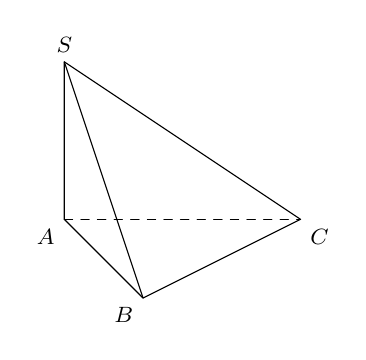
\begin{tikzpicture}[scale=1, font=\footnotesize, line join=round, line cap=round, >=stealth]
				\draw (0,0)--(1,-1)--(3,0)--(0,2)--cycle;
				\draw[dashed] (0,0)--(3,0);
				\draw (0,2)--(1,-1);
				\node[below left] at (0,0) {$A$} ;
				\node[below left]at (1,-1) {$B$} ;
				\node[below right]at (3,0) {$C$} ;
				\node[above]at (0,2) {$S$} ;
		\end{tikzpicture}}
	}
\end{ex}
%%%=============================%%%

%%%=============EX_20=============%%%
\begin{ex}%[1H8H6-1]%[Dự án D - đợt 2 NH24-25- Thy Nguyen Vo Diem]
	Cho hình chóp $S.ABCD$ có đáy $ABCD$ là hình chữ nhật, $AB=a$, $AD=a\sqrt{3}$. Cạnh bên $SA\perp(ABCD)$ và $SA=a$. Góc giữa đường thẳng $SD$ và mặt phẳng $(SAB)$ bằng
	\choice
	{$45^\circ$}
	{$90^\circ$}
	{\True $60^\circ$}
	{$30^\circ$}
	\loigiai{
		\immini{Có $\heva{&DA\perp AB\\&DA\perp SA}\Rightarrow DA\perp(SAB)$.\\
			Suy ra $SA$ là hình chiếu vuông góc của $SD$ trên $(SAB)$.\\
			Vậy $\widehat{ASD}$ là góc giữa $SD$ và $(SAB)$.\\
			Xét $\triangle SAD$ vuông tại $A$, có $\tan\widehat{ASD}=\dfrac{DA}{SA}=\dfrac{a\sqrt{3}}{a}=\sqrt{3}\Rightarrow\widehat{ASD}=60^\circ$. }{ \begin{tikzpicture}[scale=1,font=\footnotesize,line join = round, line cap = round, >= stealth]
				\coordinate (A) at (0,0);
				\def\x{2}
				\def\y{1.5}
				\def\z{2}
				\def\g{-130}% goc hbh đáy
				\def\n{90} %goc nghiêng
				\coordinate (B) at ($(A)+(\x,0)$);
				\coordinate (C) at ($(B)+(\g:\y)$);
				\coordinate (D) at ($(A)+(C)-(B)$);
				\coordinate (S) at ($(A)+(\n:\z)$);
				\coordinate (I) at ($(A)!0.5!(C)$);
				\foreach \x/\y/\z in {S/A/D,S/A/B,B/A/D}{
					\path pic[draw=red,angle radius=5pt]{right angle= \x--\y--\z};
				}
				\draw (S)--(B)--(C)--cycle;
				\draw (S)--(D)--(C);
				\draw[dashed] (S)--(A)--(B) (D)--(A) ;
				\foreach \p/\g in {A/180,B/-45,C/-45,D/-90,S/90} \draw[fill] (\p) circle(.5pt) node [shift={(\g:.3)}] {$\p$};
		\end{tikzpicture}}
	}
\end{ex}
%%%=============================%%%
\Closesolutionfile{ans}

\ind{PHẦN II.} \inden{Câu trắc nghiệm đúng sai. Trong mỗi ý a), b), c), d) ở mỗi câu, học sinh chọn đúng hoặc sai.}\\
\setcounter{ex}{0}
\Opensolutionfile{ans}[ans/1H8-Bai5-DS]
%%%=============EX_1=============%%%
\begin{ex}[Trích đề thi GKII - THPT Trần Quang Khải - BRVT - Năm học 2024-2025]%[1H8H6-1]%[Dự án D - đợt 2 NH24-25- Thy Nguyen Vo Diem]
	Cho hình chóp $S. ABCD$ có $SA\perp(ABCD)$, $SA=2a\sqrt{3}$, $ABCD$ là hình vuông cạnh bằng $2a$. Khi đó
	\choiceTF
	{\True $BD\perp(SAC)$}
	{\True $SA\perp AB$}
	{\True Gọi $H$ là hình chiếu của $A$ lên $SB$. Khi đó $AH\perp BC$}
	{Góc giữa đường thẳng $AC$ và mặt phẳng $(SBC)$ là góc $60^\circ$}
	\loigiai{
		\begin{center}
			\begin{tikzpicture}[line join=round, line cap=round, scale=0.8]
				\def\d{5} \def\r{1.8} \def\h{4} \def\l{2.2}
				
				\coordinate[label={below left}:$B$] (B) at (-3,-3);
				\coordinate[label={below right}:$C$] (C) at ($(B)+(\d,0)$);
				\coordinate[label={above left}:$A$] (A) at ($(B)+(\l,\r)$);
				\coordinate[label={above right}:$D$] (D) at ($(A)+(\d,0)$);
				\coordinate[label={above}:$S$] (S) at ($(A)+(0,\h)$);
				\coordinate[label={above left}:{$H$}] (H) at ($(S)!0.65!(B)$);
				
				\draw (S)--(B)--(C)--(D)--(S)--(C)--(H);
				\draw[dashed] (S)--(A)--(B) (A)--(D) (A)--(C) (A)--(H) (B)--(D);
				\draw
				pic[draw, angle radius=2mm]{right angle=S--A--D}
				pic[draw, angle radius=2mm]{right angle=B--A--D}
				pic[draw, angle radius=2mm]{right angle=A--H--S}
				;
				\foreach \x in {S,A,B,C,D,H}
				\draw[fill=black] (\x) circle (1pt);
			\end{tikzpicture}
		\end{center}
		\begin{itemchoice}
			\itemch Vì $BD$ vuông góc với $AC$ và $SA$ nên $BD\perp(SAC)$.
			\itemch Vì $SA\perp(ABCD)$ nên $SA\perp AB$.
			\itemch Ta có $\heva{& BC\perp AB\\
				&BC\perp SA\\}\Rightarrow BC\perp(SAB)\Rightarrow BC\perp AH$.
			\itemch 
			Kẻ $AH\perp SB$ tại $H$. Khi đó $\heva{&AH\perp SB\\&AH\perp BC}\Rightarrow AH\perp(SBC)$.\\
			Suy ra $HC$ là hình chiếu của $AC$ lên $(SBC)$.\\
			$\Rightarrow\left[AC,(SBC)\right]=(AC,HC)=\widehat{ACH}$ ($\triangle AHC$ vuông tại $H$).\\
			Ta có $AH=\dfrac{AS\cdot AB}{\sqrt{AS^2+AB^2}}=a\sqrt{3}$; $AC=2a\sqrt{2}$.\\
			Suy ra $\sin\widehat{ACH}=\dfrac{AH}{AC}=\dfrac{\sqrt{6}}{4}$.\\
			Vậy $\left[AC,(SBC)\right]\neq 60^\circ$.
		\end{itemchoice}
	}
\end{ex}
%%%=============================%%%

%%%=============EX_2=============%%%
\begin{ex}[Trích đề thi GKII - THPT Ninh Bình - Bạc Liêu - Năm học 2024-2025]%[1H8H6-1]%[Dự án D - đợt 2 NH24-25- Thy Nguyen Vo Diem]
	Cho hình chóp $S. ABCD$ có đáy $ABCD$ là hình vuông cạnh $a\sqrt{3}$, $SA$ vuông góc với đáy và $SA=a$.
	\choiceTF
	{$AC\perp(SBD)$}
	{\True Tam giác $SBC$ là tam giác vuông}
	{Góc giữa hai đường thẳng $SB$ và $CD$ là $60^\circ$}
	{\True Gọi $\beta$ là góc giữa $SC$ và mặt phẳng $(SAB)$. Khi đó $\tan\beta=\dfrac{\sqrt{3}}{2}$}
	\loigiai{
		\begin{center}
			\begin{tikzpicture}[scale=.7, font=\footnotesize,line join=round, line cap=round, >=stealth]
				\path
				(0,0) coordinate (A)
				++(-140:3) coordinate (B)
				++(0:4.5) coordinate (C)
				($(A)+(C)-(B)$) coordinate (D)
				($(A)+(0,4)$) coordinate (S)
				($(A)!1/2!(C)$) coordinate (O)
				;
				\foreach \i in{B,C,D}{\draw (S)--(\i);};
				\draw (B)--(C)--(D);
				\draw[dashed] (S)--(A)--(B) (A)--(D)--(B)
				(A)--(C) (S)--(O);
				\pic[draw,angle eccentricity=1.8,angle radius=2mm]{right angle=S--A--D};
				\foreach \i/\g in {A/180,B/-120,C/-60,D/0,S/90,O/-90}
				\fill[black] (\i) circle(1pt)+(\g:3mm)node[scale=1]{$\i$};
			\end{tikzpicture}
		\end{center}
		\begin{itemchoice}
			\itemch
			Gọi $O$ là tâm hình vuông $ABCD$.\\
			Giả sử $AC \perp (SBD)$, khi đó $AC \perp SO$ (do $SO \subset (SBD)$).\\
			Điều này là mâu thuẫn do $SA \perp AC$, mà $SA$, $SO \subset (SAC)$ nên $SO$ không thể vuông góc với $AC$.\\
			Vậy $AC$ không vuông góc với $(SBD)$.
			\itemch
			Ta có $\heva{&BC\perp AB\\&BC\perp SA}\Rightarrow BC\perp(SAB)$.\\
			Mà $SB\subset(SAB)$ nên $BC\perp SB$.\\
			Suy ra tam giác $SBC$ là tam giác vuông tại $B$.
			\itemch
			Vì $CD\parallel AB$ nên $(SB,CD)=(SB,AB)=\widehat{SBA}$.\\
			Tam giác $SAB$ vuông tại $A$, ta có $\tan\widehat{SBA}=\dfrac{SA}{AB}=\dfrac{a}{a\sqrt{3}}=\dfrac{1}{\sqrt{3}}$.\\
			Suy ra $\widehat{SBA}=30^\circ$.
			\itemch
			Vì $BC\perp(SAB)$ nên $SB$ là hình chiếu của $SC$ trên mặt phẳng $(SAB)$.\\
			Gọi $\beta$ là góc giữa $SC$ và mặt phẳng $(SAB)$.\\
			Khi đó $\beta=(SC,SB)=\widehat{BSC}$.\\
			Tam giác $SAB$ là tam giác vuông tại $A$, theo định lý Pythagoras ta có
			\[SB=\sqrt{SA^2+AB^2}=\sqrt{a^2+\left(a\sqrt{3}\right)^2}=2a.\]
			Tam giác $SBC$ là tam giác vuông tại $B$, ta có \[\tan\beta=\tan\widehat{BSC}=\dfrac{BC}{SB}=\dfrac{a\sqrt{3}}{2a}=\dfrac{\sqrt{3}}{2}.\]
		\end{itemchoice}
	}
\end{ex}
%%%=============================%%%

%%%=============EX_3=============%%%
\begin{ex}%[1H8H6-1]%[Dự án D - đợt 2 NH24-25- Thy Nguyen Vo Diem]
	Cho hình chóp $S. ABC$ có đáy $ABC$ là tam giác đều cạnh $a$. Biết $SA=a\sqrt{2}$ và $SA$ vuông góc với mặt đáy. Gọi $M$ là trung điểm của $BC$ và $H$ là hình chiếu vuông góc của $A$ lên $SM$.
	\choiceTF
	{\True Đường thẳng $AH$ vuông góc với mặt phẳng $(SBC)$}
	{\True Đường thẳng $SH$ là hình chiếu của đường thẳng $SA$ lên mặt phẳng $(SBC)$}
	{Độ dài đoạn thẳng $AH$ bằng $\dfrac{6a}{11}$}
	{Cosin góc tạo bởi đường thẳng $SA$ và mặt phẳng $(SBC)$ bằng $\dfrac{\sqrt{11}}{33}$}
	\loigiai{
		\immini{
			\begin{itemchoice}
				\itemch Vì $ABC$ là tam giác đều nên $BC\perp AM$.\\
				Lại có $BC\perp SA$, nên $BC\perp(SAM)\Rightarrow BC\perp AH$.\\
				Mặt khác $AH\perp SM$, do đó $AH\perp(SBC)$.
				\itemch Vì $AH\perp(SBC)$ nên hình chiếu của $SA$ lên $(SBC)$ là $SH$.
				\itemch $AM$ là đường trung tuyến của tam giác đều $ABC$ nên $AM=\dfrac{a\sqrt{3}}{2}$.\\
				Tam giác $SAM$ vuông tại $A$, có $AH$ là đường cao nên $$AH=\dfrac{SA\cdot AM}{\sqrt{SA^2+AM^2}}=\dfrac{a\sqrt{2}\cdot\dfrac{a\sqrt{3}}{2}}{\sqrt{2a^2+\dfrac{3a^2}{4}}}=\dfrac{a\sqrt{66}}{11}.$$
				\itemch Hình chiếu của $SA$ lên $(SBC)$ là $SH$ nên $$\cos\left(SA,(SBC)\right)=\cos(SA,SH)=\cos\widehat{ASH}=\cos\widehat{ASM}=\dfrac{SA}{SM}=\dfrac{a\sqrt{2}}{\sqrt{2a^2+\dfrac{3a^2}{4}}}=\dfrac{2\sqrt{22}}{11}.$$
			\end{itemchoice}
		}
		{
			\begin{tikzpicture}[scale=1, font=\footnotesize, line join=round, line cap=round, >=stealth]
				\def\a{3} \def\b{1.8} \def\h{2.2}
				\path
				(0:0) coordinate (A)
				(0:\a) coordinate (C)
				(-60:\b) coordinate (B)
				($(A)+(90:\h)$) coordinate (S)
				($(B)!1/2!(C)$) coordinate (M)
				($(S)!1/2.2!(M)$) coordinate (H)
				;
				\draw (S)--(A)--(B)--(C)--(S)--(B) (S)--(M);
				\draw[dashed] (A)--(C) (M)--(A)--(H);
				\foreach \x/\g in {S/90,A/180,B/-90,C/0,M/-45,H/45}
				\fill[black] (\x) circle(1pt) ($(\x)+(\g:3mm)$) node{$\x$};
				\draw pic[draw,blue,angle radius=2mm] {right angle = A--H--M};
			\end{tikzpicture}
		}
	}
\end{ex}
%%%=============================%%%

%%%=============EX_4=============%%%
\begin{ex}[Trích đề thi GKII - THPT Ngọc Lạc - Thanh Hoá - Năm học 2024-2025]%[1H8V6-3]%[Dự án D - đợt 2 NH24-25- Thy Nguyen Vo Diem]
	Cho hình chóp $S. ABC$ có đáy $ABC$ vuông cân tại $B$, $SA\perp(ABC)$, $AB=a$, \break$SA=a\sqrt{3}$.
	\choiceTF
	{\True Đường thẳng $BC$ vuông góc với đường thẳng $SB$}
	{\True Góc tạo bởi hai đường thẳng $SB$ và $AB$ bằng góc tạo bởi hai mặt phẳng $(SBC)$ và $(ABC)$}
	{Cosin góc tạo bởi hai đường thẳng $SB$ và $AB$ bằng $\dfrac{\sqrt{3}}{2}$}
	{Góc tạo bởi hai mặt phẳng $(SBC)$ và $(ABC)$ bằng $45^{\circ}$}
	\loigiai{
		\begin{center}
			\begin{tikzpicture}
				\def\a{4}
				\path 	(0:0) coordinate (A)
				(0:\a) coordinate (C)
				(-32:4*\a/5) coordinate (B)
				($(A)+(90:.9*\a)$) coordinate (S)
				($(A)!0.5!(B)$) coordinate (M);
				\draw	(A)--(B)--(C)
				(A)--(S)	(B)--(S)	(C)--(S);
				\draw[dashed] 	(A)--(C);
				\foreach \x /\goc in {A/180,B/-45,C/0,S/90}
				\fill[black] (\x) circle (1.5pt)
				($(\x)+(\goc:3mm)$) node {$\x$};
				\draw pic[draw,angle radius=2mm]{right angle=C--A--S}
				pic[draw,angle radius=5mm]{angle=S--B--A};
			\end{tikzpicture}
		\end{center}
		\begin{itemchoice}
			\itemch
			Ta có $\heva{&BC\perp SA\,(\text{do}SA\perp(ABC))\\&BC\perp AB\,(\text{do}\triangle ABC\text{vuông cân tại}B)}\Rightarrow BC\perp(SAB)$.\\
			Do đó $BC\perp SB$.
			\itemch
			Ta có $\heva{&(SBC)\cap(ABC)=BC\\&BC\perp SB\\&BC\perp AB}\Rightarrow(\big((SBC),(ABC)\big))=(SB,AB)=\widehat{SBA}$.
			\itemch
			Ta có $\big(SB,AB\big)=\widehat{SBA}$.\\
			Tam giác $SAB$ vuông tại $A$ có
			\begin{itemize}
				\item $SB=\sqrt{SA^2+AB^2}=\sqrt{\left(a\sqrt{3}\right)^2+a^2}=2a$.
				\item $\cos\widehat{SBA}=\dfrac{AB}{SB}=\dfrac{a}{2a}=\dfrac{1}{2}$.
			\end{itemize}
			Vậy cosin góc tạo bởi hai đường thẳng $SB$ và $AB$ bằng $\dfrac{1}{2}$.
			\itemch
			Ta có góc tạo bởi hai mặt phẳng $(SBC)$ và $(ABC)$ chính là $\widehat{SBA}$.\\
			Tam giác $SAB$ vuông tại $A$ có
			\begin{itemize}
				\item $SB=\sqrt{SA^2+AB^2}=\sqrt{\left(a\sqrt{3}\right)^2+a^2}=2a$.
				\item $\cos\widehat{SBA}=\dfrac{AB}{SB}=\dfrac{a}{2a}=\dfrac{1}{2}\Rightarrow\widehat{SBA}=60^\circ$.
			\end{itemize}
			Vậy góc tạo bởi hai mặt phẳng $(SBC)$ và $(ABC)$ có số bằng $60^\circ$.
		\end{itemchoice}
	}
\end{ex}
%%%=============================%%%

%%%=============EX_5=============%%%
\begin{ex}[Trích đề thi GKII - THPT Trần Cao Vân - Khánh Hòa - Năm học 2024-2025]%[1H8V6-1]%[Dự án D - đợt 2 NH24-25- Thy Nguyen Vo Diem]
	Cho hình chóp $S. ABCD$ có đáy $ABCD$ là hình vuông cạnh $a$, tâm $O$, $SO\perp(ABCD)$ và $SO=\dfrac{a\sqrt{2}}{2}$.
	\choiceTF
	{\True $SO\perp AB$}
	{Góc giữa $SB$ và $(ABCD)$ là góc $\widehat{SAB}$}
	{\True Góc giữa $SC$ và $AC$ bằng $45^\circ$}
	{Góc giữa $SO$ và $(SCD)$ là bằng $60^\circ$}
	\loigiai{
		\begin{center}
			\begin{tikzpicture}[font=\footnotesize, line join=round, line cap=round, >=stealth, scale=1]
				\path (0,0) coordinate (A)(3,0) coordinate (D) (-140:1.5) coordinate (B) ($(D)-(A)+(B)$) coordinate (C)
				($(B)!1/2!(D)$) coordinate (O)+(0,3) coordinate (S)
				($(C)!1/2!(D)$) coordinate (M)
				($(S)!(O)!(M)$) coordinate (K);
				\draw (S)--(B)--(C)--(D)--cycle (M)--(S)--(C);
				\draw[dashed] (B)--(A)--(D)--cycle (M)--(O)--(S)--(A)--(C) (O)--(K);
				\foreach \x/\g in {S/90, A/135, B/-135, C/-45, D/45, O/-90, M/-45, K/45}{\fill (\x) circle (1 pt)+(\g:0.25)node{$\x$};}
			\end{tikzpicture}
		\end{center}
		\begin{itemchoice}
			\itemch Ta có $SO\perp(ABCD)$ nên $SO\perp AB$.
			\itemch Do $SO\perp(ABCD)$ nên $O$ là hình chiếu của $S$ trên mặt phẳng $(ABCD)$.\\
			Khi đó $\left(SB,(ABCD)\right)=(SB,OB)=\widehat{SBO}$.
			\itemch Ta có $(SC,AC)=\widehat{SCA}=\widehat{SCO}$.\\
			Ta có $ABCD$ là hình vuông cạnh $a$, suy ra $OC=\dfrac{a\sqrt2}{2}$.\\
			Xét $\triangle SOC$ vuông tại $O$ ta có $SO=OC=\dfrac{a\sqrt2}{2}$ nên $\triangle SOC$ vuông cân tại $O$.\\
			Suy ra $\widehat{SCO}=45^\circ$.\\
			Vậy $(SC,AC)=45^\circ$.
			\itemch Gọi $M$ là trung điểm của cạnh $CD$.\\
			Khi đó $\heva{&CD\perp OM\subset(SOM)\\&CD\perp SO\subset(SOM)\\&OM\cap SO=O.}$\\
			Suy ra $CD\perp(SOM).$\\
			Mà $CD\subset(SCD)$ nên $(SOM)\perp(SCD)$.\\
			Ta có $(SOM)\cap(SCD)=SM$.\\
			Gọi $K\in SM$ sao cho $OK\perp SM$. Khi đó $K$ là hình chiếu của $O$ trên mặt phẳng $(SCD)$.\\
			Ta có $\left(SO,(SCD)\right)=(SO,SK)=\widehat{OSK}=\widehat{OSM}$.\\
			Xét $\triangle SOM$ vuông tại $O$ ta có
			$$\tan\widehat{OSM}=\dfrac{OM}{SO}=\dfrac{\dfrac{a}{2}}{\dfrac{a\sqrt2}{2}}=\dfrac{\sqrt2}{2}.$$
			Suy ra $\widehat{OSM}\approx 35^\circ$.
		\end{itemchoice}
	}
\end{ex}
%%%=============================%%%

\Closesolutionfile{ans}
\ind{PHẦN III.} \inden{Trả lời ngắn.}\\
\setcounter{ex}{0}
\Opensolutionfile{ans}[ans/1H8-Bai5-TLN]
%%%=============EX_1=============%%%
\begin{ex}[Trích đề thi GKII - THPT Trần Quang Khải - BRVT - Năm học 2024-2025]%[1H8V2-5]%[Dự án D - đợt 2 NH24-25- Thy Nguyen Vo Diem]
	Cho hình chóp $S. ABC$ có đáy $ABC$ là tam giác vuông tại $B$, có $AB=a$, $BC=a\sqrt{3}$. Biết $SA\perp(ABC)$, đường thẳng $SB$ tạo với đáy một góc $60^\circ$. Tính $\cos$ góc giữa $SC$ và mặt phẳng $(ABC)$ {\it (làm tròn đến hàng phần trăm)}.
	\par
	\shortans[oly]{0,76}
	\loigiai{
		\begin{center}
			\begin{tikzpicture}[scale=0.6, font=\footnotesize, line join=round, line cap=round]
				% Tọa độ các đỉnh đáy dưới
				\coordinate (A) at (0,0);
				\coordinate (B) at (2,-2);
				\coordinate (C) at (6,0);
				\coordinate (S) at (0,4);
				% Vẽ đáy dưới
				\draw (A) -- (B) -- (C) -- (S)--(A);
				\draw [dashed] (A) -- (C);
				\draw (S) -- (B);
				% Đánh nhãn các đỉnh
				\node[left] at (A) {$A$};
				\node[below] at (B) {$B$};
				\node[right] at (C) {$C$};
				\node[above] at (S) {$S$};
				\foreach \x in {S,A,B,C}{\fill (\x) circle(1pt);}
			\end{tikzpicture}
		\end{center}
		Ta có $AC=\sqrt{AB^2+BC^2}=\sqrt{a^2+(a\sqrt{3})^2}=2a$.\\
		Ta có $SA\perp (ABC)$ nên suy ra $AB$ là hình chiếu của $SB$ lên $(ABC)$ nên suy ra góc giữa $SB$ với mặt phẳng $(ABC)$ là $\widehat{SBA}=60^\circ$. Khi đó $SA=AB\cdot \tan 60^\circ=a\sqrt{3}$.\\
		Ta lại có $SC=\sqrt{SA^2+AC^2}=\sqrt{(a\sqrt{3})^2+(2a)^2}=a\sqrt{7}$.\\
		Ta có $SA\perp (ABC)$ nên suy ra $AC$ là hình chiếu của $SC$ lên $(ABC)$.\\
		Góc giữa $SC$ và mặt phẳng $(ABC)$ là óc $\widehat{SCA}$. Khi đó $\cos \widehat{SCA}= \dfrac{AC}{SC}=\dfrac{2a}{a\sqrt{7}}\approx 0,76$.
	}
\end{ex}
%%%=============================%%%

%%%=============EX_2=============%%%
\begin{ex}[Trích đề thi GKII - THPT THPT Ngọc Lạc - Thanh Hoá - Năm học 2024-2025]%[1H8V6-2]%[Dự án D - đợt 2 NH24-25- Thy Nguyen Vo Diem]
	Cho hình chóp $S. ABCD$ có đáy $ABCD$ là hình vuông cạnh $a$, $SA \perp (ABCD)$ và $SA = \dfrac{a\sqrt{2}}{2}$. Tính số đo của góc nhị diện $[S, BD, C]$ (đơn vị: độ).
	\par
	\shortans[oly]{135}
	\loigiai{
		\immini{Gọi $O$ là giao điểm của $AC$ và $BD$, khi đó $CO \perp BD$, $SO \perp B D$.\\
			Do đó, góc phẳng nhị diện $[S, B D, C]=\widehat {SOC}$.\\
			Xét $\triangle SAO$, có $A O=\dfrac{a \sqrt{2}}{2}=S A$ và góc $SAO$ là góc vuông nên tam giác $SAO$ là tam giác vuông cân tại $A$, suy ra $\widehat{SOA}=45^{\circ}$; $\widehat{SOC} =135^{\circ}$.\\
			Vậy số đo của góc nhị diện $\left[S, B D, C\right]$ bằng $135^{\circ}$.}{\begin{tikzpicture}[scale=.75, font=\footnotesize, line join=round, line cap=round, >=stealth]
				\def\a{3}
				\def\b{2.5}
				\def\h{3}
				\def\g{120}
				\path
				(0,0) coordinate (A)
				(0:\a) coordinate (D)
				--++(-\g:\b) coordinate (C)
				--++(-180:\a)coordinate (B)
				;
				\coordinate (O) at ($(A)!1/2!(C)$);
				\coordinate (S) at ($(A)+(0,\h)$);
				\coordinate (H) at ($(S)!(A)!(D)$);
				\draw (B)--(C)--(D)--(S)--(B) (S)--(C) ;
				\draw[dashed] (O)--(S)--(A)--(D)--(B)--(A)--(C) ;
				\foreach \x/\g in {A/45,B/-90,C/-90,D/0,S/90,O/-90} \fill (\x) circle (1pt)+(\g:.45)node {$\x$};
		\end{tikzpicture}}
		
	}
\end{ex}
%%%=============================%%%

%%%=============EX_3=============%%%
\begin{ex}[Trích đề thi GKII - THPT Vĩnh Linh - Quảng Trị - Năm học 2024-2025]%[1H8V6-2]%[Dự án D - đợt 2 NH24-25- Thy Nguyen Vo Diem]
	Để chuẩn bị cho đợt Hội trại 26/3 sắp tới, bạn Nam lớp 11A đã thiết kế trại theo hình vẽ sau
	\begin{center}
		\begin{tikzpicture}[scale=1.2,font=\footnotesize, line join=round, line cap=round, >=stealth]
			\coordinate (A) at (0,0);\coordinate (B) at (1,1);\coordinate (C) at (4,1);	\coordinate (D) at ($(A)+(C)-(B)$);
			\coordinate (A') at ($(A)-(0,2)$);
			\coordinate (B') at ($(A')+(B)-(A)$);
			\coordinate (C') at ($(B')+(C)-(B)$);
			\coordinate (D') at ($(A')+(D)-(A)$);
			\coordinate (N) at ($(A)!0.5!(D)$);\coordinate (E) at ($(A')!0.5!(D')$);
			\coordinate (O) at ($(C)!0.5!(A)$);\coordinate (M) at ($(C)!0.5!(D)$);
			\coordinate (S) at ($(O)+(0,1)$);
			\draw (D)--(A)--(B) (C)--(D)--(D')--(C')--(C) (A)--(A')--(D') (A)--(S)--(D) (C)--(S)--(B) (E)--(N)--(S)--(M);
			\draw[dashed] (A')--(B')--(C') (B')--(B)--(C)--(A) (B)--(D) (S)--(O)--(M) (O)--(N);
			\foreach \x/\g in {A/180,B/90,C/0,D/0,A'/-90,B'/120,C'/0,D'/-90,S/90,O/-90,M/0,N/-60,E/-90} \fill[black](\x) circle (1pt) ($(\x)+(\g:3mm)$) node{$\x$};
		\end{tikzpicture}
	\end{center}
	Cho biết $SA=SB=SC=SD$, $ABCD. A'B'C'D'$ là hình hộp chữ nhật có kích thước $AB=2{,}6$, $AD = 4{,}8$ và $AA'=2{,}3$, đồng thời góc giữa hai mặt phẳng $(SCD)$ và $(ABCD)$ bằng $30^\circ$. Tính số đo góc nhị diện $[S,AD,A']$ (số đo góc làm tròn đến hàng đơn vị của độ).
	\par
	\shortans[oly]{137}
	\loigiai{
		Gọi $O=AC\cap BD$ và $M$, $N$ lần lượt là trung điểm của $CD$, $AD \Rightarrow SO\perp (ABCD)$, $OM\perp CD$, $ON\perp AD$.\\
		Vì $\heva{&CD\perp OM\\&CD\perp SO}$ nên $CD\perp (SOM)\Rightarrow $ góc giữa hai mặt phẳng $(SCD)$ và $(ABCD)$ bằng $\widehat{SOM}$.\\
		Theo giả thiết suy ra $\widehat{SMO}=30^\circ$.\\
		Tam giác $SOM$ vuông tại $O$, ta có $SO=OM\cdot \tan 30^\circ=2{,}4\cdot \dfrac{1}{\sqrt{3}}=\dfrac{4\sqrt{3}}{5}$.\\
		Gọi $E$ là trung điểm $A'D'$, suy ra $AD\perp NE$.\\
		Vì $\heva{&AD\perp SN\\&AD\perp NE}$ nên $[S,AD,A']=\widehat{SNE}=90^\circ+\widehat{SNO}$.\\
		Tam giác $SNO$ vuông tại $O$, ta có $\tan\widehat{SNO}=\dfrac{SO}{ON}=\dfrac{\dfrac{4\sqrt{3}}{5}}{1{,3}}=\dfrac{8\sqrt{3}}{13}\Rightarrow \widehat{SNO}\approx 46{,}8^\circ$.\\
		Vậy số đo góc nhị diện $[S,AD,A']$ là $136{,}8^\circ \approx 137^{\circ}$.
	}
\end{ex}
%%%=============================%%%

%%%=============EX_4=============%%%
\begin{ex}[Trích đề thi HKII - Sở GDĐT Lạng Sơn - Năm học 2023-2024]%[1H8V6-2]%[Dự án D - đợt 2 NH24-25- Thy Nguyen Vo Diem]
	Cho hình lập phương $ABCD. A'B'C'D'$, gọi $O$ là giao điểm các đường chéo của hình lập phương đã cho. Góc nhị diện $[B, OC, D]$ có số đo bằng $\alpha$. Giá trị của $P = -34 \cos^2 \alpha + 17\cos \alpha + 2\,024$ bằng bao nhiêu?
	\par
	\shortans[oly]{2007}
	\loigiai{
		\begin{center}
			\begin{tikzpicture}[scale=0.8, font=\footnotesize, line join=round, line cap=round, >=stealth]
				%hidden: TV028
				\path
				(0,0) coordinate (A)
				++(-135:2.5) coordinate (B)
				++(0:4) coordinate (C)
				($(A)+(C)-(B)$) coordinate (D)
				;
				\foreach \i in {A,B,C,D}{\coordinate (\i') at ($(\i)+(0,4)$);
				}
				\coordinate (O) at ($(A')!1/2!(C)$) ;
				\coordinate (H) at ($(A')!2/3!(C)$) ;
				\draw (A')--(B')--(C')--(D')--cycle;
				\draw (B)--(B') (C)--(C') (D)--(D') (B)--(C)--(D) (A')--(C');
				\draw[dashed] (B)--(A)--(A') (C)--(A)--(D)--(B) (A')--(C) (A)--(C') (B)--(H)--(D) (B)--(A')--(D);
				\foreach \i/\g in {A'/135,B'/180,C'/-30,D'/45,A/150,B/-135,C/-45,D/30,O/0,H/170}
				\fill (\i) circle(1pt)+(\g:3mm) node {$\i$};
				\pic [draw,angle radius=2mm]{right angle=B--H--C}
				pic [draw,angle radius=2mm]{right angle=D--H--A'};
				\node at (0,0){\href{4AP7CZ}{\tiny \phantom{4AP7CZ}}};
			\end{tikzpicture}
		\end{center}
		Kẻ $BH\perp A'C$ ($H\in A'C$).\\
		Ta có $\heva{&BD\perp AC \\&BD\perp AA'}
		\Rightarrow BD \perp \left(ACC'A'\right)
		\Rightarrow BD \perp A'C$.\\
		Vì $\heva{&A'C \perp BD \\&A'C\perp BH}
		\Rightarrow A'C \perp (BHD)
		\Rightarrow A'C \perp BH$.\\
		Suy ra, góc nhị diện $[B,OC,D]$ là $\widehat{BHD}=\alpha$.\\
		Gọi cạnh của hình lập phương là $a$. Ta có $A'B=a\sqrt{2}$, $BD=a\sqrt{2}$.\\
		Xét tam giác $A'BC$ vuông tại $B$ ta có
		\allowdisplaybreaks
		\begin{eqnarray*}
			& & \dfrac{1}{BH^2}=\dfrac{1}{BC^2}+\dfrac{1}{BA'^2}
			=\dfrac{1}{a^2}+\dfrac{1}{\left(a\sqrt{2}\right)^2}=\dfrac{3}{2a^2}\\
			&\Rightarrow& BH=\dfrac{a\sqrt{6}}{3}.
		\end{eqnarray*}
		Xét tam giác $A'DC$ vuông tại $D$ ta có
		\allowdisplaybreaks
		\begin{eqnarray*}
			& & \dfrac{1}{DH^2}=\dfrac{1}{DC^2}+\dfrac{1}{DA'^2}
			=\dfrac{1}{a^2}+\dfrac{1}{\left(a\sqrt{2}\right)^2}
			=\dfrac{3}{2a^2}\\
			&\Rightarrow& DH=\dfrac{a\sqrt{6}}{3}.
		\end{eqnarray*}
		Xét tam giác $BHD$, theo định lí côsin ta có
		\allowdisplaybreaks
		\begin{eqnarray*}
			\cos\alpha=\cos\widehat{BHD}=\dfrac{BH^2+HD^2-BD^2}{2BH\cdot HD}
			=\dfrac{\left(\dfrac{a\sqrt{6}}{3}\right)^2+\left(\dfrac{a\sqrt{6}}{3}\right)^2-\left(a\sqrt{2}\right)^2}{2\cdot \dfrac{a\sqrt{6}}{3}\cdot \dfrac{a\sqrt{6}}{3}}
			=-\dfrac{1}{2}.
		\end{eqnarray*}
		Suy ra
		\allowdisplaybreaks
		\begin{eqnarray*}
			P = -34\cdot \left(-\dfrac{1}{2}\right)^2 + 17\cdot \left(-\dfrac{1}{2}\right) + 2\,024 = 2\,007.
		\end{eqnarray*}
	}
\end{ex}
%%%=============================%%%

%%%=============EX_5=============%%%
\begin{ex}[Trích đề thi GKII - THPT Ninh Bình-Bạc Liêu - Năm học 2024-2025]%[1H8V6-1]%[Dự án D - đợt 2 NH24-25- Thy Nguyen Vo Diem]
	\immini{Một tấm ván hình chữ nhật $ABCD$ được dùng làm mặt phẳng nghiêng để kéo một vật lên khỏi hố sâu $2$ m. Cho biết $AB = 1$ m, $AD = 3{,}5$ m. Tính góc (theo đơn vị độ) giữa đường thẳng $BD$ và đáy hố (làm tròn đến hàng phần mười).}
	{\begin{tikzpicture}[font=\footnotesize, line join=round, line cap=round, >=stealth,scale=0.85]
			\path
			(0,0) coordinate (K)
			(-2,-1) coordinate (A)
			(3,-1) coordinate (B)
			(5,0) coordinate (H)
			(0,2) coordinate (D)
			(5,2) coordinate (C)
			;
			\draw
			(D)--(A)node[above,midway,rotate=55]{$3{,}5$ m}--(B)node[below,midway,rotate=0]{$1$ m}--(H)
			(H)--(C)node[right,midway,rotate=0]{$2$ m}--(D)--(B)--(C);
			\draw [dashed] (D)--(K)--(H) (A)--(K);
			\pic[draw,angle radius=1.5mm,angle eccentricity=1.5] {right angle = C--H--B};
			\foreach \x/\g in
			{K/150,A/180,B/-30,H/0,D/90,C/90}
			\fill[black](\x) circle (1pt)
			($(\x)+(\g:3mm)$) node{$\x$};
	\end{tikzpicture}}
	\par
	\shortans[oly]{33,3}
	\loigiai{
		Gọi mặt phẳng đáy hố là $(P)$. Đây là mặt phẳng nằm ngang.
		Theo đề bài, tấm ván $ABCD$ là hình chữ nhật nên $AB \perp AD$.
		Kích thước tấm ván là $AB = 1$ m, $AD = 3{,}5$ m.\\
		Áp dụng định lý Pythagore trong tam giác vuông $ABD$, ta có độ dài đường chéo của tấm ván:
		\[ BD^2 = AB^2 + AD^2 = 1^2 + (3{,}5)^2 = 1 + 12{,}25 = 13{,}25\Rightarrow BD = \sqrt{13{,}25} \text{ m}. \]
		Gọi $K$ là hình chiếu vuông góc của $D$ lên mặt phẳng đáy hố $(P)$.\\
		Vì hố sâu $2$ m nên khoảng cách thẳng đứng từ $D$ xuống mặt phẳng đáy hố là $DK = 2$ m.\\
		Hình chiếu của đường thẳng $BD$ lên mặt phẳng đáy hố $(P)$ là đường thẳng $BK$.\\
		Góc $\alpha$ giữa đường thẳng $BD$ và mặt phẳng đáy hố $(P)$ chính là góc giữa $BD$ và hình chiếu $BK$, tức là $\alpha = \widehat{DBK}$.\\
		Xét tam giác $\triangle DBK$ vuông tại $K$, ta có
		$\sin\alpha= \dfrac{KD}{BD} = \dfrac{2}{\sqrt{13{,}25}}$.\\
		Suy ra
		$\alpha \approx 33{,}3^\circ$.
	}
\end{ex}
%%%=============================%%%

\Closesolutionfile{ans}
\ind{PHẦN IV.} \inden{Tự luận.}\\
\setcounter{ex}{0}
%%%=============EX_1=============%%%
\begin{ex}%[1H8H6-2]%[Dự án D - đợt 2 NH24-25- Thy Nguyen Vo Diem]
	Cho hình chóp $S.ABCD$ có đáy $ABCD$ là hình thoi cạnh $a$. Cạnh $SA=\dfrac{a}{2}$ và vuông góc với mặt đáy. Tính số đo góc nhị diện $[S,CD,A]$.
	\loigiai{
		\immini{
			Gọi $H$ là hình chiếu vuông góc của $A$ trên $CD$. \\
			Khi đó $AH\perp CD$.\\
			Vì $SA\perp(ABCD)$ nên $SA\perp CD$. Suy ra $CD\perp(SAH)$.\\
			Khi đó $SH\perp CD$. \\
			Như vậy, số đo của $[S,CD,A]=\widehat{SHA}$.\\
			Ta có $AH=\dfrac{a\sqrt{3}}{2}; SA=\dfrac{a}{2}$ nên $\tan\widehat{SHA}=\dfrac{SA}{AH}=\dfrac{\sqrt{3}}{3}$.\\
			Vậy số đo của $[S,CD,A]=\widehat{SHA}=30^\circ$.
		}{
			\begin{tikzpicture}[line join=round,line cap=round,line width=.6pt,font=\footnotesize,scale=.9]
				\coordinate[label=below: $B$] (B) at (0,0);
				\coordinate[label=above right:$A$] (A) at (1.2,1.2);
				\coordinate[label=below: $C$] (C) at (4,0);
				\coordinate[label=above right:$D$] (D) at ($(C)-(B)+(A)$);
				\coordinate (O) at ($(A)!.5!(C)$);
				\coordinate[label=below:$H$] (H) at ($(D)!.5!(C)$);
				\coordinate[label=above left:$S$] (S) at ($(O)+(90:3)$);
				\draw (B)--(C)--(D)--(S)--cycle (S)--(C);
				\draw (S)--(H);
				\draw[dashed] (C)--(A)--(D) (S)--(A)--(B);
				\draw[dashed] (A)--(H)--(B);
				\fill (A)circle(1.5pt) (B)circle(1.5pt) (C)circle(1.5pt) (D)circle(1.5pt) (S)circle(1.5pt) (H)circle(1.5pt);
			\end{tikzpicture}
		}
	}
\end{ex}
%%%=============================%%%

%%%=============EX_2=============%%%
\begin{ex}%[Trích đề thi GKII - THPT Edison - Hải Phòng - Năm học 2024-2025]%[1H8H6-1]%[Dự án D - đợt 2 NH24-25- Thy Nguyen Vo Diem]
	Cho hình chóp $S.ABC$ có $SA$ vuông góc với mặt phẳng $(ABC)$, $SA=2a$, tam giác $ABC$ vuông cân tại $B$ và $AB=a\sqrt{2}$. Góc giữa đường thẳng $SC$ và mặt phẳng $(ABC)$ bằng bao nhiêu độ?
	\loigiai{
		\immini{
			Ta có $SA\perp(ABC)$ nên $A$ là hình chiếu vuông góc của $S$ lên $(ABC)$.\\
			Do đó $\left(SC,(ABC)\right)=\widehat{SCA}$.\\
			Xét $\triangle ABC$ vuông cân tại $B$, ta có
			$$ AC=\sqrt{AB^2+BC^2}=\sqrt{\left(a\sqrt{2}\right)^2+\left(a\sqrt{2}\right)^2}=2a. $$
			Xét $\triangle SAC$ vuông tại $A$, ta có
			$$\tan\widehat{SCA}=\dfrac{SA}{AC}=\dfrac{2a}{2a}=1\Rightarrow\widehat{SCA}=45^\circ. $$
			Vậy $\left(SC,(ABC)\right)=\widehat{SCA}=45^\circ$.
		}{
			\begin{tikzpicture}[font=\footnotesize,line join=round, line cap=round, >=stealth,scale=1]
				\path
				(0,0) coordinate (A)
				(1.7,-1.7) coordinate (B)
				(3.4,0) coordinate (C)
				(0,3.2) coordinate (S)
				;
				\draw (S)--(A)--(B)--(C)--(S)--(B);
				\draw[dashed] (A)--(C);
				\foreach \x/\g in {A/180, B/-90, C/-45, S/90} \fill (\x) circle(1pt) node[{shift=(\g:0.3)}]{$\x$};
				\foreach \a/\b/\c in {S/A/B, S/A/C, A/B/C} {\draw pic [draw, angle radius=2mm] {right angle=\a--\b--\c};}
				\draw pic [draw, angle radius=5mm] {angle=S--C--A};
			\end{tikzpicture}
		}
	}
\end{ex}
%%%=============================%%%

%%%=============EX_3=============%%%
\begin{ex}%[Trích đề thi GKII - THPT Lê Lợi Kon Tum - Năm học 2024-2025]%[1H8H6-1]%[Dự án D - đợt 2 NH24-25- Thy Nguyen Vo Diem]
	Cho hình chóp $S.ABC$ có đáy là tam giác vuông cân tại $C$, $SA\perp(ABC)$, biết $SA=2$, $AC=1$. Tính tang góc giữa đường thẳng $SB$ và mặt phẳng đáy (làm tròn kết quả đến hàng phần trăm).
	%\shortans[oly]{1{,}41}
	\loigiai{
		\immini
		{
			Ta có $SA\perp(ABC)$ nên $AB$ là hình chiếu vuông góc của $SB$ trên mặt phẳng $(ABC)$.\\
			Suy ra góc giữa $SB$ và mặt đáy là góc giữa $SB$ và $AB$ là góc $\widehat{SBA}=\alpha$.\\
			Xét $\triangle ABC$ vuông cân tại $C$ ta có $AB=\sqrt{1^2+1^2}=\sqrt{2}$.\\
			Xét tam giác $SAB$ vuông tại $A$ ta có $\tan\alpha=\dfrac{SA}{AB}=\dfrac{2}{\sqrt{2}}=\sqrt{2}\approx 1{,}41$.
		}
		{
			\begin{tikzpicture}[scale=0.7, font=\footnotesize, line join=round, line cap=round, >=stealth]
				\def\ac{4} % cạnh AC
				\def\ab{2} % cạnh AB
				\def\h{3} % chiều cao
				\def\gocA{50} % góc A của đáy
				\coordinate[label=left:$A$] (A) at (0,0);
				\coordinate[label=right:$C$] (C) at (\ac,0);
				\coordinate[label=below left:$B$] (B) at (-\gocA:\ab);
				\coordinate[label=above:$S$] (S) at ($(A)+(90:\h)$);
				% \coordinate[label=above right:$H$] (H) at ($(S)!0.5!(B)$);
				\draw (A)--(B)--(C)--(S)--(A) (S)--(B);
				\draw[dashed] (A)--(C);
				\foreach \diem in {A,B,C,S}	\fill (\diem)circle(1pt);
				\newcommand{\gocv}[4][black]{\draw[#1] ($(#3)!5pt!(#2)$)--($(#3)!2!($($(#3)!5pt!(#2)$)!.5!($(#3)!5pt!(#4)$)$)$)--($(#3)!5pt!(#4)$);}
				\gocv{S}{A}{C}
			\end{tikzpicture}
		}
	}
\end{ex}
%%%=============================%%%

%%%=============EX_4=============%%%
\begin{ex}%[1H8V6-1]%[Trích đề thi GKII - THPT Phan Đình Phùng - Hà Nội - Năm học 2024-2025]%[1H8H6-1%[Dự án D - đợt 2 NH24-25- Thy Nguyen Vo Diem]
	Cho hình chóp $S.ABC$ có đáy là tam giác vuông cân tại $B$ và $SA\perp(ABC)$.
	\begin{enumerate}
		\item Chứng minh tam giác $SBC$ là tam giác vuông.
		\item Biết rằng $AB=AS=a$, tính góc giữa đường thẳng $SB$ với mặt phẳng $(SAC)$.
	\end{enumerate}
	\loigiai{
		\immini{
			\begin{enumerate}
				\item
				Ta có $\heva{&BC\perp AB\\&BC\perp SA\,(\text{do $SA \perp (ABC)$})}\Rightarrow BC\perp(SAB)$.\\
				Do $SB\subset(SAB)$ nên $BC\perp SB$, suy ra tam giác $SBC$ vuông tại $B$.
				\item Gọi $M$ là trung điểm của $AC$. \\
				Do tam giác $ABC$ vuông cân tại $B$ nên $BM\perp AC$. \\
				Ta có $\heva{&BM\perp AC\\&BM\perp SA\,(\text{do $SA \perp (ABC)$})}\Rightarrow BM\perp(SAC)$.\\
				Suy ra $M$ là hình chiếu của $B$ trên $(SAC)$.\\
				Khi đó $(SB,(SAC))=(SB,SM)=\widehat{BSM}$.\\
				Ta có $AC=a\sqrt{2}$, do đó $BM=\dfrac{1}{2}AC=\dfrac{a\sqrt{2}}{2}$, và $SB=a\sqrt{2}$.\\
				Suy ra $\sin\widehat{BSM}=\dfrac{BM}{SB}=\dfrac{1}{2}\Rightarrow\widehat{BSM}=30^\circ$.
			\end{enumerate}
		}
		{
			\begin{tikzpicture}[declare function={goc=-45; a=4.5; b=0.45*a; h=3.5;}]
				\path
				(0,0) coordinate (A)--+(0,h) coordinate (S)
				(a,0) coordinate (C)
				(goc:b) coordinate (B)
				($(A)!0.5!(C)$) coordinate (M);
				\draw
				pic[angle radius=3mm,draw] {right angle = S--A--C}
				pic[angle radius=3mm,draw] {right angle = S--A--B}
				pic[angle radius=3mm,draw] {right angle = C--B--A}
				;
				\draw[dashed] (A)--(C) (S)--(M)--(B);
				\draw (S)--(B) (S)--(A)--(B)--(C)--cycle;
				\foreach \x/\goc in {S/90,A/240,C/-60,B/-90,M/45}
				\fill (\x) node[shift={(\goc:7pt)},font=\scriptsize]{$\x$} circle (1pt);
			\end{tikzpicture}
		}
		
	}
\end{ex}
%%%=============================%%%

%%%=============EX_5=============%%%
\begin{ex}%[Trích đề thi GKII - THPT Trần Cao Vân- Khánh Hòa - Năm học 2024-2025]%[1H8H6-1]%[Dự án D - đợt 2 NH24-25- Thy Nguyen Vo Diem]
	Cho hình chóp $S.ABCD$ có đáy $ABCD$ là hình chữ nhật, với $SA=AB=a$, $AD=a\sqrt{2}$, $SA\perp(ABCD)$. Gọi $H$ là hình chiếu vuông góc của $A$ trên $SD$.
	\begin{itemize}
		\item[a)] Chứng minh $AH\perp(SCD)$.
		\item[b)] Tính góc giữa đường thẳng $SC$ và mặt phẳng $(ABCD)$.
	\end{itemize}
	\loigiai{
		\begin{center}
			\begin{tikzpicture}[scale=1, font=\footnotesize, line join=round, line cap=round, >=stealth]
				\def\a{3}
				\coordinate (B) at (0,0);
				\coordinate (C) at (\a*1.2,0);
				\coordinate (A) at ($(B)+(\a*0.5,\a*0.5)$);
				\coordinate (D) at ($(A)+(C)-(B)$);
				\coordinate (S) at ($(A)+(0,\a)$);
				\coordinate (H) at ($(S)!1/3!(D)$);
				\draw (S)--(B)--(C)--(D)--(S)--(C);
				\draw[dashed] (B)--(A)--(D) (S)--(A)--(H);
				\foreach \x/\label/\g in {A/$A$/180, B/$B$/180, C/$C$/0, D/$D$/0, S/$S$/90, H/$H$/0}{
					\fill (\x) circle (1pt);
					\node at ($(\x)+(\g:3mm)$) {\small \label};
				};
				\pic [draw, angle radius=3mm] {right angle=A--H--S};
			\end{tikzpicture}
		\end{center}
		\textbf{a)} Chứng minh rằng $AH\perp(SCD)$.\\
		Thật vậy,
		\[\heva{
			&CD\perp AD\ (\text{do } ABCD\text{ là hình chữ nhật})\\
			&CD\perp SA\ (\text{do } SA\perp (ABCD))\\
			&AD\subset (SAD)\\
			&SA\subset (SAD)\\
			&AD\ \text{cắt } SA
		}
		\Rightarrow CD\perp (SAD)
		\Rightarrow CD\perp AH\quad (1).
		\]
		Ta có
		\[\heva{
			&AH\perp CD\ (\text{theo (1)})\\
			&AH\perp SD\ (\text{giả thiết})\\
			&CD\subset (SCD)\\
			&SD\subset (SCD)\\
			&CD\ \text{cắt } SD
		}
		\Rightarrow AH\perp (SCD).
		\]
		\textbf{b)} Tính góc giữa $SC$ và mặt phẳng $(ABCD)$.\\
		Thật vậy,
		$SA\perp(ABCD)$ nên hình chiếu vuông góc của $SC$ trên $(ABCD)$ là $AC$.\\
		Suy ra, góc giữa $SC$ và $(ABCD)$ là góc $\widehat{SCA}$.\\
		Xét tam giác $SAC$ vuông tại $A$ có $SA=a$,	$AC=\sqrt{AB^2+BC^2}=\sqrt{a^2+\big(a\sqrt{2}\big)^2}=a\sqrt{3}$.
		\[\tan \widehat{SCA}=\dfrac{SA}{AC}=\dfrac{a}{a\sqrt{3}}=\dfrac{1}{\sqrt{3}}
		\Rightarrow \widehat{SCA}=30^\circ.
		\]
		Vậy góc giữa đường thẳng $SC$ và mặt phẳng $(ABCD)$ có số đo bằng $30^\circ$.
	}
\end{ex}
%%%=============================%%%

%%%=============EX_6=============%%%
\begin{ex}%[1H8V6-2]%[Dự án D - đợt 2 NH24-25- Thy Nguyen Vo Diem]
	Cho hình chóp $S.ABCD$ có $AC$ cắt $BD$ tại $O$. Gọi $\alpha$, $\beta$ lần lượt là số đo của các nhị diện $[A,SO,B]$ và $[B,SO,C]$. Tính $\alpha+\beta$.
	\loigiai{
		\immini
		{
			Trong mặt phẳng $(SAC)$, lấy đường thẳng $AN$ $(N\in SC)$ sao cho $AN\perp SO$.\\
			Gọi $M$ là giao điểm của $AN$ và $SO$.\\
			Trong mặt phẳng $(SOB)$, lấy đường thẳng $MP\perp SO$.\\
			Khi đó, số đo của $[A,SO,B]$ bằng $\widehat{AMP}$, hay $\widehat{AMP}=\alpha$ và số đo của $[B,SO,C]$ bằng $\widehat{PMN}$, hay $\widehat{PMN}=\beta$.\\
			Trong mặt phẳng $(APN)$ có $A$, $M$, $N$ thẳng hàng nên $\alpha+\beta=180^{\circ}$.
		}
		{
			\begin{tikzpicture}[scale=0.8, font=\footnotesize,line join=round, line cap=round, >=stealth]
				\coordinate (A) at (0,0);
				\coordinate (D) at (-2,-2);
				\coordinate (B) at (4.5,0);
				\coordinate (C) at (4,-3.5);%($(B)+(D)-(A)$);
				\coordinate (S) at ($(A)+(0,4)$);
				\coordinate (N) at ($(S)!0.7!(C)$);
				\coordinate (P) at ($(S)!0.7!(B)$);
				\path (intersection of A--C and B--D) coordinate (O)
				(intersection of S--O and A--N) coordinate (M);
				\foreach \i in {B,C,D}{\draw (S)--(\i);}
				\draw (B)--(C)--(D);
				\draw[dashed,thin](S)--(A)--(C) (B)--(A)--(D)--cycle (S)--(O) (A)--(N) (M)--(P);
				%\pic[draw,thin,angle radius=3mm] {right angle = S--A--D} pic[draw,thin,angle radius=3mm] {right angle = S--A--B};
				\foreach \i/\g in {S/90,A/180,B/0,C/-90,D/180,O/-90,N/0,M/0,P/30}{\draw[fill=black](\i) circle (1.0pt) ($(\i)+(\g:3mm)$) node[scale=1]{$\i$};}
			\end{tikzpicture}
		}
	}
\end{ex}
%%%=============================%%%

%%%=============EX_7=============%%%
\begin{ex}%[Trích đề thi GKII - THPT Edison - Hải Phòng - Năm học 2024-2025]%[1H8V6-2]%[Dự án D - đợt 2 NH24-25- Thy Nguyen Vo Diem]
	Cho hình hộp chữ nhật $ABCD.A'B'C'D'$ có cạnh đáy bằng $a$, cạnh bên bằng $a\sqrt{3}$. Xác định và tính côsin của góc phẳng nhị diện $\left[C',AB,D\right]$.
	\loigiai{
		\immini{
			Ta có $AB\perp(BCC'B')$ mà $C'B\subset(BCC'B')\Rightarrow C'B\perp AB$.\\
			Vì $(ABCD)$ là nửa mặt phẳng chứa điểm $D$, bờ là đường thẳng $AB$.\\
			Hơn nữa, ta có $BC\subset(ABCD)$ và $BC\perp AB\Rightarrow\widehat{C'BC}$ là góc nhị diện $\left[C',AB,D\right]$.\\
			Xét $\triangle CBC'$ vuông tại $C$, ta có
			$$ BC'=\sqrt{BC^2+CC'^2}=\sqrt{a^2+3a^2}=2a. $$
			Ta có $\cos\widehat{CBC'}=\dfrac{BC}{BC'}=\dfrac{a}{2a}=\dfrac{1}{2}$.
		}{
			\begin{tikzpicture}[font=\footnotesize,line join=round, line cap=round, >=stealth,scale=0.8]
				\path
				(0,0) coordinate (A)
				(4,0) coordinate (B)
				(-1.1,-1.4) coordinate (D)
				($(B)-(A)+(D)$) coordinate (C)
				(0,3) coordinate (x)
				($(A)+(x)$) coordinate (A')
				($(B)+(x)$) coordinate (B')
				($(C)+(x)$) coordinate (C')
				($(D)+(x)$) coordinate (D')
				;
				\fill[yellow!30] (A)--(C')--(B)--cycle;
				\fill[red!5] (A)--(B)--(C)--(D)--cycle;
				\draw (D')--(D)--(C)--(B)--(B')--(A')--(D')--(C')--(B') (C)--(C')--(B);
				\draw[dashed] (A')--(A)--(B) (D)--(A)--(C');
				\foreach \x/\g in {A/180, B/0, C/-90, D/-90,A'/90,B'/90,C'/135,D'/135} \fill (\x) circle(1pt) node[{shift=(\g:0.3)}]{$\x$};
				\foreach \a/\b/\c in {C'/B/C} {\draw pic [draw, angle radius=3mm] {angle=\a--\b--\c};}
			\end{tikzpicture}
		}
	}
\end{ex}
%%%=============================%%%

%%%=============EX_8=============%%%
\begin{ex}%[1H8V6-1]%[Dự án D - đợt 2 NH24-25- Thy Nguyen Vo Diem]
	Cho hình chóp $S.ABCD$, gọi $\alpha_1$, $\alpha_2$, $\alpha_3$, $\alpha_4$ lần lượt là góc giữa các đường thẳng $SA$, $SB$, $SC$, $SD$ với mặt phẳng $(ABCD)$. Chứng minh rằng $SA=SB=SC=SD\Leftrightarrow\alpha _1=\alpha _2=\alpha _3=\alpha _4$.
	\loigiai{
		\begin{center}
			\begin{tikzpicture}[scale=.8, font=\footnotesize, line join=round, line cap=round, >=stealth]
				\def\bc{5}
				\def\ba{3}
				\def\h{4.5}
				\def\gocB{30}
				\coordinate[label=below left:$B$] (B) at (0,0);
				\coordinate[label=above right:$A$] (A) at (\gocB:\ba);
				\coordinate[label=below:$C$] (C) at (\bc,0);
				\coordinate[label=right:$D$] (D) at ($(C)-(B)+(A)-(0.3,0.3)$);
				\coordinate[label=below:$H$] (H) at (2,0.6);
				\coordinate[label=above:$S$] (S) at ($(H)+(90:\h)$);
				\draw (B)--(C)--(D)--(S)--cycle (B)--(S)--(C);
				\draw[dashed] (H)--(A)--(D) (S)--(A)--(B)--(H)--(C) (S)--(H)--(D);
				\foreach \diem in {A,B,C,D,S,H}	\fill (\diem)circle(1.5pt);
			\end{tikzpicture}
		\end{center}
		Gọi $H$ là hình chiếu của $S$ lên mặt phẳng $(ABCD)$. Khi đó
		$$\alpha _1=\widehat{SAH},\,\alpha _2=\widehat{SBH},\,\alpha _3=\widehat{SCH},\,\alpha _4=\widehat{SDH}.$$
		Xét các tam giác vuông $SAH$, $SBH$, $SCH$, $SDH$ có chung cạnh góc vuông $SH$.
		Khi đó
		$$SA=SB=SC=SD\Leftrightarrow\Delta SAH=\Delta SBH=\Delta SCH=\Delta SDH\Leftrightarrow\alpha _1=\alpha _2=\alpha _3=\alpha _4.$$
	}
\end{ex}
%%%=============================%%%

%%%=============EX_9=============%%%
\begin{ex}%[1H8V6-2]%[Dự án D - đợt 2 NH24-25- Thy Nguyen Vo Diem]
	Cho hình chóp $S. ABC$ có $SA\perp(ABC)$, $AB\perp BC$, $SA=AB=3a$, $BC=4a$. Gọi $\alpha$, $\beta$, $\gamma$ lần lượt là số đo của các góc nhị diện $[B, SA, C]$, $[A, BC, S]$, $[A, SC, B]$. Tính
	\begin{enumerate}
		\item $\cos\alpha,\cos\beta$;
		\item $\cos\gamma$.
	\end{enumerate}
	\loigiai{
		\immini{
			\begin{enumerate}
				\item Vì $SA\perp(ABC)$, $AB\subset(ABC)$, $AC\subset(ABC)$ nên $SA\perp AB$, $SA\perp AC$. Suy ra góc $BAC$ là góc phẳng nhị diện của $[B, SA, C]$, hay $\widehat{BAC}=\alpha$. Xét tam giác $ABC$ vuông tại $B$ có
				\[A C=\sqrt{A B^2+B C^2}=\sqrt{(3 a)^2+(4 a)^2}=5 a. \]
				và $\cos\alpha=\cos\widehat{BAC}=\dfrac{BA}{AC}=\dfrac{3a}{5a}=\dfrac{3}{5}$.\\
				Ta có $BC\perp(SAB)$ nên $BC\perp SB$ suy ra góc $SBA$ là góc phẳng nhị diện của $[A, BC, S]$. Như vậy, ta có
				\[S B=\sqrt{A B^2+S A^2}=\sqrt{(3 a)^2+(3 a)^2}=3 \sqrt{2} a. \]
				và $\cos\beta=\cos\widehat{SBA}=\dfrac{AB}{SB}=\dfrac{3a}{3\sqrt{2}a}=\dfrac{\sqrt{2}}{2}$.
			\end{enumerate}
		}{
			\begin{tikzpicture}[>=stealth,line join=round,line cap=round,font=\footnotesize,scale=1]
				\def\a{5};
				\def\b{2};
				\def\g{-40};
				\def\cao{4};
				\path
				(0,0) coordinate (A)
				(0:\a) coordinate (C)
				(\g:\b) coordinate (B)
				($(A)+(90:\cao)$) coordinate (S)
				($(S)!0.4!(B)$) coordinate (H)
				($(S)!0.6!(C)$) coordinate (K)
				;
				\draw (S)--(A)--(B)--(C)--(S)--(B) (A)--(H)--(K);
				\draw[dashed] (A)--(C) (A)--(K);
				\foreach \x/\g in {A/180,B/-90,C/0,S/90,H/45,K/30}\fill[black](\x) circle (1pt) +(\g:3mm) node {$\x$};
				\pic[draw,angle radius=2mm]{right angle=A--B--C};
				\pic[draw,angle radius=2mm]{right angle=A--H--S};
				\pic[draw,angle radius=2mm]{right angle=A--K--S};
			\end{tikzpicture}
		}
		\begin{enumerate}
			\setcounter{enumi}{1}
			\item Gọi $H$, $K$ lần lượt là hình chiếu của $A$ trên $SB$, $SC$. Ta có $BC\perp(SAB)$ nên $BC\perp AH$. Mà $AH\perp SB$ nên $AH\perp(SBC)$, suy ra $AH\perp SC$. Mà $SC\perp AK$ nên $SC\perp(AHK)$, suy ra $SC\perp HK$. Do đó góc $AKH$ là góc phẳng nhị diện của $[A, SC, B]$, hay $\widehat{AKH}=\gamma$.\\
			Tam giác $SAB$ vuông tại $A$ có $AH=\dfrac{SA\cdot AB}{SB}=\dfrac{3a\cdot 3a}{3a\sqrt{2}}=\dfrac{3a}{\sqrt{2}}$.\\
			Tam giác $SAC$ vuông tại $A$ có $AK=\dfrac{SA\cdot AC}{SC}=\dfrac{3a\cdot 5a}{\sqrt{(3a)^2+(5a)^2}}=\dfrac{15a}{\sqrt{34}}$.\\
			Tam giác $AHK$ vuông tại $H($ vì $AH\perp(SBC)$ mà $HK\subset(SBC))$ có
			\[H K=\sqrt{A K^2-A H^2}=\sqrt{\left(\dfrac{15 a}{\sqrt{34}}\right)^2-\left(\dfrac{3 a}{\sqrt{2}}\right)^2}=\dfrac{6 a}{\sqrt{17}}. \]
			và $\cos\gamma=\cos\widehat{AKH}=\dfrac{HK}{AK}=\dfrac{\dfrac{6a}{\sqrt{17}}}{\dfrac{15a}{\sqrt{34}}}=\dfrac{2\sqrt{2}}{5}$.
		\end{enumerate}
	}
\end{ex}
%%%=============================%%%

%%%=============EX_10=============%%%
\begin{ex}%[1H8V6-2]%[Dự án D - đợt 2 NH24-25- Thy Nguyen Vo Diem]
	Cho hình chóp $S.ABCD$ có $ABCD$ là hình vuông, $AC$ cắt $BD$ tại $O$, $SO\perp(ABCD)$. Tất cả các cạnh của hình chóp bằng $a$.
	\begin{enumerate}
		\item Tính góc giữa đường thẳng $SB$ và mặt phẳng $(SAC)$.
		\item Gọi $\alpha$ là số đo của góc nhị diện $[S,CD,A]$. Tính $\cos\alpha$.
		\item Gọi $d$ là giao tuyến của hai mặt phẳng $(SAB)$ và $(SCD)$, $\beta$ là số đo của góc nhị diện $[A,d,D]$. Tính $\cos\beta$.
		\item Gọi $\gamma$ là số đo của góc nhị diện $[B,SC,D]$. Tính $\cos\gamma$.
	\end{enumerate}
	\loigiai{
		\immini{
			\begin{enumerate}
				\item Vì $BO\perp AC, BO\perp SO$ nên $BO\perp(SAC)$.\\
				Suy ra góc giữa đường thẳng $SB$ và mặt phẳng $(SAC)$ bằng góc $BSO$.\\
				Xét tam giác $SBD$ có $SB=SD$ và $SB^2+SD^2=BD^2$ nên tam giác $SBD$ vuông cân tại $S$.\\
				Suy ra $\widehat{BSO}=45^\circ$, hay góc giữa đường thẳng $SB$ và mặt phẳng $(SAC)$ bằng $45^\circ$.
				\item Gọi $N$ là hình chiếu của $S$ trên $CD$. Khi đó, số đo của $[S, CD, A]$ bằng $\widehat{SNO}$, hay $\widehat{SNO}=\alpha$.\\
				Ta có
				\[\cos \alpha=\dfrac{O N}{S N}=\dfrac{\dfrac{a}{2}}{\dfrac{a \sqrt{3}}{2}}=\dfrac{\sqrt{3}}{3}. \]
			\end{enumerate}
		}{
			\begin{tikzpicture}[>=stealth,line join=round,line cap=round,font=\footnotesize,scale=1]
				\def\a{6};
				\def\b{2};
				\def\g{35};
				\def\cao{5.5};
				\path
				(0,0) coordinate (B)
				(0:\a) coordinate (C)
				(\g:\b) coordinate (A)
				($(A)+(C)-(B)$) coordinate (D)
				($(A)!0.5!(C)$) coordinate (O)
				($(O)+(90:\cao)$) coordinate (S)
				($(A)!0.5!(B)$) coordinate (M)
				($(C)!0.5!(D)$) coordinate (N)
				($(S)!0.5!(C)$) coordinate (H)
				($(S)+(A)-(B)$) coordinate[label=above:$d$] (d)
				;
				\draw (C)--(S)--(B)--(C)--(D)--(S)--(N) (B)--(H)--(D) (d)--($(d)!2!(S)$);
				\draw[dashed] (O)--(S)--(A)--(B)--(D)--(A)--(C) (S)--(M)--(N);
				\foreach \x/\g in {A/30,B/-135,C/-35,D/0,S/90,H/35,M/180,N/-10,O/-90}\fill[black](\x) circle (1pt) +(\g:3mm) node {$\x$};
				\pic[draw,angle radius=2mm]{right angle=S--M--A};
				\pic[draw,angle radius=2mm]{right angle=S--N--D};
				\pic[draw,angle radius=2mm]{right angle=B--H--C};
			\end{tikzpicture}
		}
		\begin{enumerate}
			\setcounter{enumi}{2}
			\item Gọi $M$ là hình chiếu của $S$ trên $AB$.\\
			Vì $AB\parallel CD$ nên $d\parallel AB$ và $d\parallel CD$. Khi đó $SM\perp d$, $SN\perp d$.\\
			Suy ra số đo của $[A, d, D]$ bằng $\widehat{MSN}$, hay $\widehat{MSN}=\beta$.\\
			Ta có
			\[\cos \beta=\dfrac{S M^2+S N^2-M N^2}{2 S M \cdot S N}=\dfrac{\left(\dfrac{a \sqrt{3}}{2}\right)^2+\left(\dfrac{a \sqrt{3}}{2}\right)^2-a^2}{2 \cdot \dfrac{a \sqrt{3}}{2} \cdot \dfrac{a \sqrt{3}}{2}}=\dfrac{1}{3}. \]
			\item Gọi $H$ là hình chiếu của $B$ trên $SC$, khi đó $BH \perp SC$.\\
			Vì $BD\perp(SAC)$ nên $BD\perp SC$. Suy ra $SC\perp(BHD)$ nên $SC\perp HD$.\\
			Vậy số đo của $[B, SC, D]$ bằng $\widehat{BHD}$, hay $\widehat{BHD}=\gamma$.\\
			$\triangle SBC$ và $\triangle SDC$ là các tam giác đều có đường cao lần lượt là $BH$ và $HD$ nên $BH=HD=\dfrac{a\sqrt{3}}{2}$.\\
			$BD$ là đường chéo hình vuông $ABCD$ cạnh $a$ nên $BD=a\sqrt{2}$.\\
			Áp dụng định lí cosin trong $\triangle BHD$, ta có \[\cos \widehat{BHD}=\cos \gamma=\dfrac{HB^2+HD^2-BD^2}{2\cdot HB \cdot HD}=\dfrac{\left(\dfrac{a\sqrt{3}}{2}\right)^2+\left(\dfrac{a\sqrt{3}}{2}\right)^2-\left(a\sqrt{2}\right)^2}{2\cdot \dfrac{a\sqrt{3}}{2} \cdot \dfrac{a\sqrt{3}}{2}}=-\dfrac{1}{3}.\]
		\end{enumerate}
	}
\end{ex}
%%%=============================%%%


